%%
% Copyright (c) 2017, Pascal Wagler;  
% Copyright (c) 2014--2017, John MacFarlane
% Modifications by Paul Bauriegel 2018 and Lars Dittert 2019
% 
% All rights reserved.
% 
% Redistribution and use in source and binary forms, with or without 
% modification, are permitted provided that the following conditions 
% are met:
% 
% - Redistributions of source code must retain the above copyright 
% notice, this list of conditions and the following disclaimer.
% 
% - Redistributions in binary form must reproduce the above copyright 
% notice, this list of conditions and the following disclaimer in the 
% documentation and/or other materials provided with the distribution.
% 
% - Neither the name of John MacFarlane nor the names of other 
% contributors may be used to endorse or promote products derived 
% from this software without specific prior written permission.
% 
% THIS SOFTWARE IS PROVIDED BY THE COPYRIGHT HOLDERS AND CONTRIBUTORS 
% "AS IS" AND ANY EXPRESS OR IMPLIED WARRANTIES, INCLUDING, BUT NOT 
% LIMITED TO, THE IMPLIED WARRANTIES OF MERCHANTABILITY AND FITNESS 
% FOR A PARTICULAR PURPOSE ARE DISCLAIMED. IN NO EVENT SHALL THE 
% COPYRIGHT OWNER OR CONTRIBUTORS BE LIABLE FOR ANY DIRECT, INDIRECT, 
% INCIDENTAL, SPECIAL, EXEMPLARY, OR CONSEQUENTIAL DAMAGES (INCLUDING,
% BUT NOT LIMITED TO, PROCUREMENT OF SUBSTITUTE GOODS OR SERVICES; 
% LOSS OF USE, DATA, OR PROFITS; OR BUSINESS INTERRUPTION) HOWEVER 
% CAUSED AND ON ANY THEORY OF LIABILITY, WHETHER IN CONTRACT, STRICT 
% LIABILITY, OR TORT (INCLUDING NEGLIGENCE OR OTHERWISE) ARISING IN 
% ANY WAY OUT OF THE USE OF THIS SOFTWARE, EVEN IF ADVISED OF THE 
% POSSIBILITY OF SUCH DAMAGE.
%%

%%
% For usage information and examples visit the GitHub page of this template:
% https://github.com/Wandmalfarbe/pandoc-latex-template
%%

\PassOptionsToPackage{unicode=true}{hyperref} % options for packages loaded elsewhere
\PassOptionsToPackage{hyphens}{url}
%
\documentclass[12pt,english,a4paper,oneside,,tablecaptionabove]{scrbook}
\usepackage{dblfloatfix}
\usepackage{helvet}
\renewcommand{\familydefault}{\sfdefault}
\usepackage{setspace}
\setstretch{1.5}
\usepackage{acronym}
\usepackage{graphicx}
\usepackage{subfig}

\usepackage{longtable}

\usepackage{amssymb,amsmath}
\usepackage{ifxetex,ifluatex}
\usepackage{floatrow}
\usepackage{fixltx2e} % provides \textsubscript
\ifnum 0\ifxetex 1\fi\ifluatex 1\fi=0 % if pdftex
  \usepackage[T1]{fontenc}
  \usepackage[utf8]{inputenc}
  \usepackage{textcomp} % provides euro and other symbols
\else % if luatex or xelatex
  \usepackage{unicode-math}
  \defaultfontfeatures{Ligatures=TeX,Scale=MatchLowercase}
\fi
% use upquote if available, for straight quotes in verbatim environments
\IfFileExists{upquote.sty}{\usepackage{upquote}}{}
% use microtype if available
\IfFileExists{microtype.sty}{%
\usepackage[]{microtype}
\UseMicrotypeSet[protrusion]{basicmath} % disable protrusion for tt fonts
}{}
\IfFileExists{parskip.sty}{%
\usepackage{parskip}
}{% else
\setlength{\parindent}{0pt}
\setlength{\parskip}{6pt plus 2pt minus 1pt}
}
\usepackage{hyperref}
\hypersetup{
            pdftitle={Technical and organizational challenges when adopting DevOps principles for the integration of Artificial Intelligence into classical Software Engineering},
            pdfauthor={Pascal Schroeder},
            pdfkeywords={AI, ML, DevOps, AIOps, Kubernetes, Kubeflow},
            pdfborder={0 0 0},
            breaklinks=true}
\urlstyle{same}  % don't use monospace font for urls
\usepackage[margin=2.5cm,bottom=2.5cm,headsep=0.5cm,footskip=0.8cm,includehead=true,includefoot=true,centering]{geometry}
\usepackage{listings}
\newcommand{\passthrough}[1]{#1}
\usepackage{graphicx,grffile}
\makeatletter
\def\maxwidth{\ifdim\Gin@nat@width>\linewidth\linewidth\else\Gin@nat@width\fi}
\def\maxheight{\ifdim\Gin@nat@height>\textheight\textheight\else\Gin@nat@height\fi}
\makeatother
% Scale images if necessary, so that they will not overflow the page
% margins by default, and it is still possible to overwrite the defaults
% using explicit options in \includegraphics[width, height, ...]{}
\setkeys{Gin}{width=\maxwidth,height=\maxheight,keepaspectratio}
\setlength{\emergencystretch}{3em}  % prevent overfull lines
\providecommand{\tightlist}{%
  \setlength{\itemsep}{0pt}\setlength{\parskip}{0pt}}
\setcounter{secnumdepth}{3}
% Redefines (sub)paragraphs to behave more like sections
\ifx\paragraph\undefined\else
\let\oldparagraph\paragraph
\renewcommand{\paragraph}[1]{\oldparagraph{#1}\mbox{}}
\fi
\ifx\subparagraph\undefined\else
\let\oldsubparagraph\subparagraph
\renewcommand{\subparagraph}[1]{\oldsubparagraph{#1}\mbox{}}
\fi

% Make use of float-package and set default placement for figures to H
\usepackage{float}
\floatplacement{figure}{H}

\makeatletter
\@ifpackageloaded{subfig}{}{\usepackage{subfig}}
\@ifpackageloaded{caption}{}{\usepackage{caption}}
\captionsetup[subfloat]{margin=0.5em}
\AtBeginDocument{%
\renewcommand*\figurename{Figure}
\renewcommand*\tablename{Table}
}
\AtBeginDocument{%
\renewcommand*\listfigurename{List of Figures}
\renewcommand*\listtablename{List of Tables}
}
\newcommand*\listoflistings\lstlistoflistings
\AtBeginDocument{%
\renewcommand*{\lstlistlistingname}{List of Listings}
}
\makeatother
\ifnum 0\ifxetex 1\fi\ifluatex 1\fi=0 % if pdftex
  \usepackage[shorthands=off,main=english]{babel}
\else
    % See issue https://github.com/reutenauer/polyglossia/issues/127
  \renewcommand*\familydefault{\sfdefault}
    % load polyglossia as late as possible as it *could* call bidi if RTL lang (e.g. Hebrew or Arabic)
  \usepackage{polyglossia}
  \setmainlanguage[]{english}
\fi

\title{Technical and organizational challenges when adopting DevOps principles
for the integration of Artificial Intelligence into classical Software
Engineering}
\author{Pascal Schroeder}
\providecommand{\institute}[1]{}
\institute{Duale Hochschule Baden-Württemberg}
\date{}





%%
%% added
%%

%
% No language specified? take American English.
%


%
% colors
%
\usepackage[dvipsnames,svgnames*,x11names*,table]{xcolor}

%
% listing colors
%
\definecolor{listing-background}{HTML}{F7F7F7}
\definecolor{listing-rule}{HTML}{B3B2B3}
\definecolor{listing-numbers}{HTML}{B3B2B3}
\definecolor{listing-text-color}{HTML}{000000}
\definecolor{listing-keyword}{HTML}{435489}
\definecolor{listing-identifier}{HTML}{435489}
\definecolor{listing-string}{HTML}{00999A}
\definecolor{listing-comment}{HTML}{8E8E8E}
\definecolor{listing-javadoc-comment}{HTML}{006CA9}

%\definecolor{listing-background}{rgb}{0.97,0.97,0.97}
%\definecolor{listing-rule}{HTML}{B3B2B3}
%\definecolor{listing-numbers}{HTML}{B3B2B3}
%\definecolor{listing-text-color}{HTML}{000000}
%\definecolor{listing-keyword}{HTML}{D8006B}
%\definecolor{listing-identifier}{HTML}{000000}
%\definecolor{listing-string}{HTML}{006CA9}
%\definecolor{listing-comment}{rgb}{0.25,0.5,0.35}
%\definecolor{listing-javadoc-comment}{HTML}{006CA9}

%
% for the background color of the title page
%
\usepackage{pagecolor}
\usepackage{afterpage}

%
% TOC depth and 
% section numbering depth
%
\setcounter{tocdepth}{3}
\setcounter{secnumdepth}{3}

%
% line spacing
%

%
% break urls
%
\PassOptionsToPackage{hyphens}{url}

%
% When using babel or polyglossia with biblatex, loading csquotes is recommended 
% to ensure that quoted texts are typeset according to the rules of your main language.
%
\usepackage{csquotes}

%
% captions
%
\definecolor{caption-color}{HTML}{777777}
\usepackage[font={stretch=1.2}, textfont={color=caption-color}, position=top, skip=4mm, labelfont=bf, singlelinecheck=false, justification=raggedright]{caption}
\setcapindent{0em}
\captionsetup[longtable]{position=above}

%
% blockquote
%
\definecolor{blockquote-border}{RGB}{221,221,221}
\definecolor{blockquote-text}{RGB}{119,119,119}
\usepackage{mdframed}
\newmdenv[rightline=false,bottomline=false,topline=false,linewidth=3pt,linecolor=blockquote-border,skipabove=\parskip]{customblockquote}
\renewenvironment{quote}{\begin{customblockquote}\list{}{\rightmargin=0em\leftmargin=0em}%
\item\relax\color{blockquote-text}\ignorespaces}{\unskip\unskip\endlist\end{customblockquote}}

%
% Source Sans Pro as the de­fault font fam­ily
% Source Code Pro for monospace text
%
% 'default' option sets the default 
% font family to Source Sans Pro, not \sfdefault.
%
\usepackage[default]{sourcesanspro}
\usepackage{sourcecodepro}
\usepackage[export]{adjustbox}

%
% heading color
%
\definecolor{heading-color}{RGB}{40,40,40}
\addtokomafont{section}{\color{heading-color}}
% When using the classes report, scrreprt, book, 
% scrbook or memoir, uncomment the following line.
%\addtokomafont{chapter}{\color{heading-color}}

%
% variables for title and author
%
\usepackage{titling}
\title{Technical and organizational challenges when adopting DevOps principles
for the integration of Artificial Intelligence into classical Software
Engineering}
\author{Pascal Schroeder}

%
% tables
%

%
% remove paragraph indention
%
\setlength{\parindent}{0pt}
\setlength{\parskip}{6pt plus 2pt minus 1pt}
\setlength{\emergencystretch}{3em}  % prevent overfull lines

%
%
% Listings
%
%

\lstdefinestyle{eisvogel_listing_style}{
  language         = java,
  numbers          = left,
  backgroundcolor  = \color{listing-background},
  basicstyle       = \color{listing-text-color}\small\ttfamily{}\linespread{1.15}, % print whole listing small
  xleftmargin      = 2.7em,
  breaklines       = true,
  frame            = single,
  framesep         = 0.6mm,
  rulecolor        = \color{listing-rule},
  frameround       = ffff,
  framexleftmargin = 2.5em,
  tabsize          = 4,
  numberstyle      = \color{listing-numbers},
  aboveskip        = 1.0em,
  keywordstyle     = \color{listing-keyword}\bfseries,
  classoffset      = 0,
  sensitive        = true,
  identifierstyle  = \color{listing-identifier},
  commentstyle     = \color{listing-comment},
  morecomment      = [s][\color{listing-javadoc-comment}]{/**}{*/},
  stringstyle      = \color{listing-string},
  showstringspaces = false,
  escapeinside     = {/*@}{@*/}, % Allow LaTeX inside these special comments
  literate         =
  {á}{{\'a}}1 {é}{{\'e}}1 {í}{{\'i}}1 {ó}{{\'o}}1 {ú}{{\'u}}1
  {Á}{{\'A}}1 {É}{{\'E}}1 {Í}{{\'I}}1 {Ó}{{\'O}}1 {Ú}{{\'U}}1
  {à}{{\`a}}1 {è}{{\'e}}1 {ì}{{\`i}}1 {ò}{{\`o}}1 {ù}{{\`u}}1
  {À}{{\`A}}1 {È}{{\'E}}1 {Ì}{{\`I}}1 {Ò}{{\`O}}1 {Ù}{{\`U}}1
  {ä}{{\"a}}1 {ë}{{\"e}}1 {ï}{{\"i}}1 {ö}{{\"o}}1 {ü}{{\"u}}1
  {Ä}{{\"A}}1 {Ë}{{\"E}}1 {Ï}{{\"I}}1 {Ö}{{\"O}}1 {Ü}{{\"U}}1
  {â}{{\^a}}1 {ê}{{\^e}}1 {î}{{\^i}}1 {ô}{{\^o}}1 {û}{{\^u}}1
  {Â}{{\^A}}1 {Ê}{{\^E}}1 {Î}{{\^I}}1 {Ô}{{\^O}}1 {Û}{{\^U}}1
  {œ}{{\oe}}1 {Œ}{{\OE}}1 {æ}{{\ae}}1 {Æ}{{\AE}}1 {ß}{{\ss}}1
  {ç}{{\c c}}1 {Ç}{{\c C}}1 {ø}{{\o}}1 {å}{{\r a}}1 {Å}{{\r A}}1
  {€}{{\EUR}}1 {£}{{\pounds}}1 {«}{{\guillemotleft}}1
  {»}{{\guillemotright}}1 {ñ}{{\~n}}1 {Ñ}{{\~N}}1 {¿}{{?`}}1
  {…}{{\ldots}}1 {≥}{{>=}}1 {≤}{{<=}}1 {„}{{\glqq}}1 {“}{{\grqq}}1
  {”}{{''}}1
}
\lstset{style=eisvogel_listing_style}

\lstdefinelanguage{XML}{
  morestring      = [b]",
  moredelim       = [s][\bfseries\color{listing-keyword}]{<}{\ },
  moredelim       = [s][\bfseries\color{listing-keyword}]{</}{>},
  moredelim       = [l][\bfseries\color{listing-keyword}]{/>},
  moredelim       = [l][\bfseries\color{listing-keyword}]{>},
  morecomment     = [s]{<?}{?>},
  morecomment     = [s]{<!--}{-->},
  commentstyle    = \color{listing-comment},
  stringstyle     = \color{listing-string},
  identifierstyle = \color{listing-identifier}
}

%
% header and footer
%
\usepackage{fancyhdr}
\pagestyle{fancy}
\fancyhead{}
\fancyfoot{}
\lhead{Pascal Schroeder - Bachelor Thesis}
\chead{}
\rhead{}
\lfoot{}
\cfoot{\thepage}
\rfoot{}
\renewcommand{\headrulewidth}{0.4pt}
\renewcommand{\footrulewidth}{0pt}

%%
%% end added
%%

\begin{document}

%%
%% begin titlepage
%%

\begin{titlepage}
\newgeometry{margin=2.5cm,bottom=1cm,headsep=0.5cm,footskip=0.5cm,includehead=true,includefoot=true,centering}
\begin{longtable}{p{0.5\textwidth} p{0.5\textwidth}}

\includegraphics[height=1.5cm, left]{images/logo.png}&

\includegraphics[height=1.5cm, right]{images/dhbw.png}
\end{longtable}
\newcommand{\colorRule}[3][black]{\textcolor[HTML]{#1}{\rule{#2}{#3}}}
\noindent
\makebox[0pt][s]{\colorRule[1f70c1]{1.04\textwidth}{1pt}}
\par
\noindent

{ \setstretch{1.4}
\vskip 4em
\begin{center}
\noindent {{\Large \textbf{\textsf{Technical and organizational challenges when adopting DevOps principles
for the integration of Artificial Intelligence into classical Software
Engineering}}}}
\vskip 1em
{\large \textsf{\textbf{Bachelor Thesis}}}
\vskip 2em
{\large \textsf{for the degree of}}
\vskip 1em
{\large \textsf{Bachelor of Science}}
\vskip 1em
{\large \textsf{from the Course of Studies Applied Computer Science}}
\vskip 1em
{\large \textsf{at the Cooperative State University Baden-Württemberg Mannheim}}
\vskip 2em
{\large \textsf{by}}
\vskip 1em
{\large \textsf{Pascal Schroeder}}
\end{center}
\begin{figure}[b!]
\begin{flushleft} 
\begin{tabular}{l l}
\textsf{\textbf{Time of Project}:} & \textsf{01/07/2019 - 23/09/2019}\\

\textsf{\textbf{Student ID, Course}:} & \textsf{5501463, TINF16AI-BC}\\

\textsf{\textbf{Company}:}  & \textsf{IBM Deutschland GmbH, Ehningen}\\

\textsf{\textbf{Supervisor in the Company}:} & \textsf{Steffen Krause}\\

\textsf{\textbf{Reviewer in Corporate State University}:} & \textsf{Prof.~Dr.~Holger Hofmann}\\
\noindent
\end{tabular}
\end{flushleft}
\end{figure}
}
\end{titlepage}
\restoregeometry


%%
%% end titlepage
%%




 % Erklärung
\thispagestyle{empty}
\pagenumbering{gobble}
\addchap*{Declaration of Sincerity}

\normalsize Hereby I solemnly declare that my project report, titled \textit{Technical and organizational challenges when adopting DevOps principles
for the integration of Artificial Intelligence into classical Software
Engineering} is
independently authored and no sources other than those specified have been used.
\\I also declare that the submitted electronic version matches the printed version.\\\\

\vspace{3em}
Mannheim, 23rd September, 2019
\vspace{4em}

\rule{6cm}{0.4pt}\\
Pascal Schroeder
\newpage



\newpage
\pagestyle{plain}
\setcounter{page}{1}
\pagenumbering{Roman}

{
\setcounter{tocdepth}{2}
\tableofcontents
}
% Abbildungsverzeichnis
	\cleardoublepage
	\listoffigures

%Tabellenverzeichnis

% Quellcodeverzeichnis
	\cleardoublepage
	\lstlistoflistings
\addchap*{Abkürzungsverzeichnis}
\begin{acronym}
	\acro{AI}[AI]{Artificial Intelligence}
	\acro{IT}[IT]{Information Technology}
	\acro{DevOps}[DevOps]{Development and Operations}
	\acro{API}[API]{Application Programming Interface}
	\acro{REST}[REST]{Representional State Transfer}
	\acro{SaaS}[SaaS]{Software as a Service}
	\acro{ML}[ML]{Machine Learning}
	\acro{VM}[VM]{Virtual Machine}
	\acro{CPU}[CPU]{Central Processing Unit}
	\acro{GPU}[GPU]{Graphics Processing Unit}
	\acro{IDE}[IDE]{Integrated Development Environment}
	\acro{ANN}[ANN]{Artificial Neural Network}
	\acro{CRISP-DM}[CRISP-DM]{Cross Industry Standard Process for Data Mining}
\end{acronym}

\newpage
\pagestyle{fancy}
\pagenumbering{arabic}
\setcounter{page}{1}
\hypertarget{sec:intro}{%
\chapter{Introduction - Software Development Trends}\label{sec:intro}}

The upcoming trends of \acl{AI} (\acs{AI}) and Cloud Computing are
changing the world of \acl{IT} (\acs{IT}) as a whole. One very important
aspect is the way applications are developed and operated. These
processes can be summarized under the term \acl{DevOps} (\acs{DevOps}).
This work will deal with how AI and Cloud force DevOps to transform and
will discuss different approaches to adopt and realize those principles
for AI applications. The following chapter will introduce the terms of
AI and Cloud computing and will describe how these innovations force
DevOps to transform.

\hypertarget{sec:devchanges}{%
\section{Changes in Software Development caused by
AI}\label{sec:devchanges}}

First discussed in the 1940s, Artificial Intelligence has made great
progress in recent years thanks to advances in computing capacity as
well as Deep Neural networks and the accessibility of huge amounts of
data. {[}\protect\hyperlink{ref-JanakiramMSV}{1}{]} This leads to
companies investing in AI about 32€ Billion in 2019 according to a
forecast by IDC, which makes it one of the most important fields of
businesses. {[}\protect\hyperlink{ref-MichaelShirer}{2}{]}

These progresses do not only impact the products itself, but also their
development. In contrast to a traditional software development process
in which the business logic is explicitly encoded in rules, solutions
that rely on \acl{ML} (\acs{ML}) are fed with huge amounts of data that
contains the business logic only implicitly.

This leads to a completely different development cycle. While classical
software development is focused on the design and the development of the
code, which is followed by testing and deployment, the machine learning
lifecycle consists out of data collection, preparation, the training of
the model with those data as well as the deployment of this model.
{[}\protect\hyperlink{ref-MariyaYao}{3}{]} The differences between both
is described in more detail in chapter \ref{sec:devopsai}.

This new type of software development is getting more and more
important. Some people like Andrej Karpathy, Director of AI at Tesla,
even predict, that these new type of software will replace traditional
software development as a whole.
{[}\protect\hyperlink{ref-AndrejKarpathy}{4}{]} This has some
advantages, e.g.~that it is easier to learn and to manage, more
homogeneous and very well portable. In return it is harder to understand
for humans so that those systems appear to us as \enquote{black boxes}.
Also debugging can be very difficult as well because usually there is no
real error message. {[}\protect\hyperlink{ref-MariyaYao}{3}{]}

In this work, all the progresses that have led to this transformation
will be explained in more detail. Additionally, it will be described
which difficulties and challenges come along with it, focused on
necessary changes for operations of the development cycle, called
DevOps.

\hypertarget{sec:cloud}{%
\section{Cloud Computing}\label{sec:cloud}}

In 2009 the university of Berkeley published a paper, in which the
potential of Cloud Computing has been discussed. In doing so Cloud
Computing has been defined as both - the applications delivered as
services over the Internet, referred to as \acl{SaaS} (\acs{SaaS}), as
well as the hardware and the systems software in the datacenters that
provide those services.
{[}\protect\hyperlink{ref-ArmbrustA.FoxandR.Griffith2009}{5}{]}

Thereby a distinction is made between a Public Cloud and a Private
Cloud. A Cloud is called public when it is made available in a
pay-as-you-go manner to the public. This means, that you pay for a
service in advance and then you can only use what you have paid for.
Private Cloud on the other hand refers to internal datacenters of a
business or other organizations unavailable to the public.
{[}\protect\hyperlink{ref-ArmbrustA.FoxandR.Griffith2009}{5}{]}

SaaS in general has advantages for both end-users as well as service
providers. While the service provider can install, maintain and control
their services more easily, the user can access the service anytime,
anywhere, collaborate more easily and keep their data inside the
infrastructure.
{[}\protect\hyperlink{ref-ArmbrustA.FoxandR.Griffith2009}{5}{]}

Cloud Computing enables this possibility to more application providers
and additionally also the possibility to scale their applications on
demand. Based on this possibility there are some more advantages
identified for Cloud Computing in particular:

\begin{itemize}
\tightlist
\item
  The illusion of infinite computing resources on demand
\item
  The elimination of an up-front commitment by Cloud users
\item
  The ability to pay for use of computing resources
  {[}\protect\hyperlink{ref-ArmbrustA.FoxandR.Griffith2009}{5}{]}
\end{itemize}

The first point eliminates the need to plan far ahead how many resources
are needed but enables the user to buy as many resources as necessary as
soon as it is needed.

Also, Cloud users are allowed to change their need for resources any
time, so they can scale up their application and don't have to commit to
their need beforehand as described in point two.

The last point is about saving money when the resources are no longer
needed. As it is possible to scale up, it is also possible to scale
down, which eliminates the need to pay for the resources. This relieves
the Cloud users from taking too much risk when paying for resources they
may not need for a long time.

For realizing those advantages different approaches were competing with
each other: One looking similar to physical hardware with the ability to
control the entire software stack similar to a low-level \acl{VM}
(\acs{VM}). The alternative was a clean separation between a stateless
computation tier and a stateful storage tier. In this competition, the
first option has become established, because in the beginning most users
wanted to recreate their local environment instead of writing new
programs solely for the cloud.
{[}\protect\hyperlink{ref-Jonas2019}{6}{]}

But this solution still forced the User to manage their environment
themselves. Especially for simpler applications, it is desirable to have
an easier path to deploy their applications to the Cloud.

Amazon provisioned a new solution for those needs in 2015 called AWS
Lambda. Lambda offered the possibility to simply write the code to be
executed and leaves all server provisioning and administration tasks to
the cloud provider. {[}\protect\hyperlink{ref-Amazon}{7}{]}

This is known as serverless computing, because - even though there are
still servers being used for the computation tasks - the user does not
have to care about any tasks on serverside and can focus on writing the
code. Serverless services must scale and bill automatically based on
usage without any need for explicit provisioning.
{[}\protect\hyperlink{ref-Jonas2019}{6}{]}

Those new possibilities with the Cloud technology changed the way of how
developers can deploy and manage their products. Additionally, also AI
development benefit from this very strongly because of several reasons.

The first one is automated scalability, which eliminates the need to
worry about raising workloads. Additionally, when AI models are being
trained, there are many resources needed, but besides this task, there
are not as many resources necessary. Through serverless computing, this
idle time will not be billed.
{[}\protect\hyperlink{ref-BhagyashreeR}{8}{]}

Serverless computing also reduces the interdependence, because the
functions can be updated, deleted or invoked any time without having any
side effect on the rest of the system.
{[}\protect\hyperlink{ref-BhagyashreeR}{8}{]}

All this forced developers to change their way of developing and
operating their products. This change of the DevOps lifecycle will be
introduced in chapter \ref{sec:devopsai}

\hypertarget{sec:devopsai}{%
\section{Development Operations in time of AI}\label{sec:devopsai}}

The traditional software development has continuously been improving for
years, defining standards and principles to increase the efficiency,
portability, and quality of the development cycle. Those principles and
practices are called DevOps. In the new type of software development
described in chapter \ref{sec:devchanges}, not all of those are
applicable any more and new ones need to be defined. Additionally, the
upcoming Cloud technology changed the way how products can be deployed
and managed as described in chapter \ref{sec:cloud}. In this chapter,
the consequences of those changes for DevOps will be examined.

Starting with development itself and ending with maintaining and
improving the product, there are DevOps principles for every single
stage of the development cycle. This is described in more detail in
chapter \ref{sec:devops}. In the new world of AI and Cloud, those stages
are different, some new stages have been added, others have become
unnecessary.

A short, simplified comparison between the required steps of traditional
operations and Machine Learning operations can be seen in figure
\ref{fig:img}.

\begin{figure}
\hypertarget{fig:img}{%
\centering
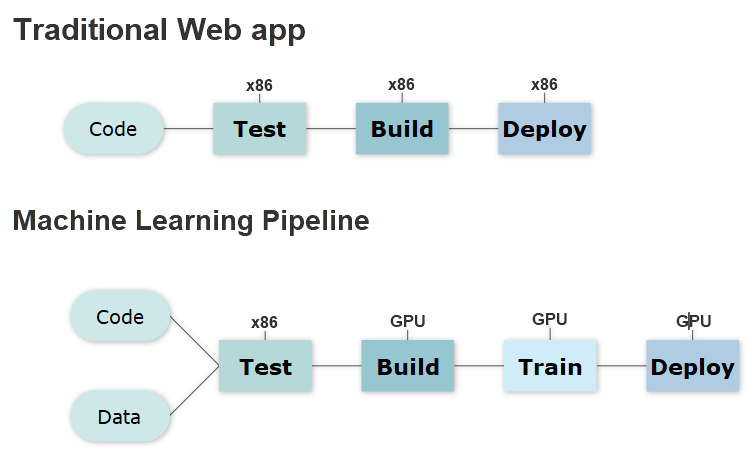
\includegraphics[width=4.16667in,height=\textheight]{images/chapter1/traditional_ml_comp.png}
\caption{Comparison development lifecycle traditional app and ML
pipeline{[}\protect\hyperlink{ref-Dillon}{9}{]}}\label{fig:img}
}
\end{figure}

In traditional development, there is one input - the code. This code has
to be tested, built and then deployed.

The Machine Learning pipeline looks different. First, there is an
additional input - data, which is very important for Machine Learning
applications. The code and the data still need to be tested afterward.

Also, it needs to be built. The difference in this stage is, that the
resources used for building an ML application are usually different.
While traditional applications are usually built on regular \acs{CPU}s
(\acl{CPU}), Machine Learning pretty much rely on \acs{GPU}s
(\acl{GPU}), which leads to a more heterogeneous and complex hardware
landscape.

A third difference is the training step. ML applications have to be fed
with training data. This step can take very long especially when
insufficient hardware is being used.

The last differentiator is, that ML pipelines are continuously updated
with new data. This process is called \enquote{refitting} the model.

Besides the rise of AI, Cloud Computing also changed the way of how
products are deployed and managed. The Cloud can serve as a centralized
platform for testing, deployment, and production. Also, it can
automatically scale applications and allocate needed resources.
Serverless computing even eliminates the need to set up a complete
system and offers a simple way to deploy Machine Learning or other
functions. {[}\protect\hyperlink{ref-DavidLinthicum}{10}{]}

AI tools on the other hand are enabling new possibilities for improving
the IT operations functions like monitoring, analysis, service
management, and automation.

All those progresses led to two big trends in the DevOps area. The first
one is using Artificial Intelligence for DevOps. In doing so Machine
Learning functionalities are used to enhance all IT operations. Gartner
calls this \enquote{AIOps} and predicts, that the use of AIOps will rise
from 5\% in 2018 to 30\% in 2023.
{[}\protect\hyperlink{ref-SusanMoore2019}{11}{]}

The second trend is using DevOps for the development of AI. This means
adopting existing principles and practices for the traditional
development cycle to the development cycle of AI tools. The objective of
this is to upheld existing standards and maximize the efficiency of the
development processes. {[}\protect\hyperlink{ref-Dillon}{9}{]}

In this work this second trend will be analyzed, the influences leading
to it will be described and possible solutions will be shown, compared
and discussed.

\hypertarget{sec:theory}{%
\chapter{Theory - DevOps, Cloud and Machine Learning}\label{sec:theory}}

In this chapter, the theoretical basis, that is needed for creating
DevOps principles for AI, will be given. For that, it will be started
with an explanation of what DevOps is in general. Then it will be shown,
which new possibilities came with Cloud and 12-factor-apps in chapter
\ref{sec:ms12}. After that, the basics of Machine Learning and AI will
be given in chapter \ref{sec:ml}, specializing on the lifecycle of AI
development in chapter \ref{sec:aicycle}. Last in chapter
\ref{sec:devopsai}, all these knowledge will be combined to adopt the
DevOps principles explained in chapter \ref{sec:devops} to the new world
of AI with the help of Cloud technologies.

\hypertarget{sec:devops}{%
\section{Development Operations}\label{sec:devops}}

Since people started manufacturing products on a mass scale, the goal is
to increase the efficiency of this manufacturing process and reduce
waste of time and material.

One early set of best practices for manufacturing was the concept of
\emph{Lean manufacturing}, which tries to reduce the waste of resources
and time of a production cycle as much as possible. With the upcoming
use of software as a commercial product in the 1970s
{[}\protect\hyperlink{ref-Pugh:2002:OSB:513126.513131}{12}{]} a desire
came on to create best practices for developing and operating products
the same way as it was already usual in conventional manufacturing.
{[}{\textbf{???}}{]}

In 2009 two Flickr employees - John Allspaw and Paul Hammond - presented
their way of combining Development and Operations. Inspired by this
presentation, a Belgian consultant named Patrick Debois formed a new
conference - the \enquote{Devopsday} in Ghent. This naming is how the
term \enquote{DevOps} has been created and prevailed.
{[}\protect\hyperlink{ref-SteveMezak}{13}{]}

Since then, DevOps has been established or at least planned in 91\% of
all companies as an essential way to increase their efficiency of
software development. {[}\protect\hyperlink{ref-SauceLabs}{14}{]} For
almost every stage of development, there are principles and practices
defined and continuously improved. However, before those practices are
explained, further insight into the business need will be given. All
this will be oriented to the book \enquote{DevOps for Dummies} by
Sanjeev Sharma and Bernie Coyne.
{[}\protect\hyperlink{ref-Sharma2017}{15}{]}

Every process or product need a business value that covers the costs
caused by it. For that, there must be either an outcome for the customer
or reduced producing costs.

For DevOps, it is usually even both - on the one hand, enhanced customer
experience can be guaranteed, and on the other hand, the efficiency of
the production cycle can be increased.

One example of enhanced customer experience are practices to get fast
feedback from all stakeholders. This feedback can then be used to
improve the designed product. One of such practices is the so-called
\enquote{A-B testing}. There, two different sets of features are
enrolled in two groups of randomly chosen users. Both can give their
feedback to the producer, and the set with better feedback will then
later be enrolled for every user.

The efficiency can be increased through reduced waste and rework with
practices to write reusable components. Other examples are tools for
planning a product or fast ways to deliver a product without the need to
redeploy everything step by step. In this chapter, the advantages of
DevOps will be delighted in more detail, and some of the practices will
be described and explained.

\hypertarget{principles}{%
\subsection{Principles}\label{principles}}

The DevOps movement is generally based on four principles. The first one
is to \emph{develop and test against production-like systems} to move
operations concerns earlier in the life cycle. The purpose of this is to
see how the system behaves and performs before it gets deployed. This is
also advantageous from an operations perspective, because it can be
seen, how the system behaves when it supports the application.

The second principle is to \emph{deploy with repeatable and reliable
processes}. The objective is to create a delivery pipeline, that enables
continuous, automated deployment and testing of the product.

Third, it is crucial to \emph{monitor and validate operational quality.}
This means that applications and systems should not only be monitored in
production, but already earlier. This forces automated testing to be
done early and often to monitor the application. Metrics should always
be captured and analyzed to provide an early warning system about
potential issues and risks.

The last principle is to \emph{amplify feedback loops} intending to
enable a quick reaction to issues. For this, organizations need to
create a communication channel to their users, so that they can give
feedback, and the developers can react to it accordingly.

\hypertarget{practices}{%
\subsection{Practices}\label{practices}}

The DevOps practices that have become commonplace can be split into four
different sets based on the different periods of a product lifecycle. To
each set, there are several practices, standards, and tools available,
which help to achieve the best possible result. The four different sets
and some example practices can be seen in figure
\ref{devops_architecture}.

\begin{figure}
\hypertarget{fig:devops_architecture}{%
\centering
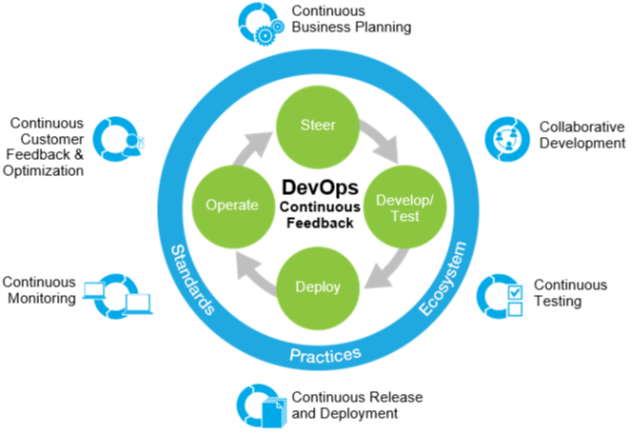
\includegraphics[width=4.16667in,height=\textheight]{images/chapter2/devops_architecture.png}
\caption{DevOps reference
architecture{[}\protect\hyperlink{ref-Sharma2017}{15}{]}}\label{fig:devops_architecture}
}
\end{figure}

The first set is called \textbf{Steer}, which is about managing and
planning the development and lifecycle of a product. This set includes
establishing and continuously adjusting business goals. The process of
resolving this issue is called \emph{Continuous Business Planning}.

This practice includes three major points - the acceleration of software
delivery, a good balance between speed, cost, quality and risk, and the
reduction of the time it needs to get customer feedback.
{[}\protect\hyperlink{ref-IBM2013}{16}{]}

These points are mainly fulfilled via tools and practices to track the
status, feedback, and needs of a project efficiently. First, a vision of
the projects overall objective should be created, and every action
should be guided by it. {[}\protect\hyperlink{ref-IBM2013}{16}{]}

The strategy, which should lead to this vision, has to be monitored and
adjusted continuously based on new information and feedback. This
procedure is called \emph{continuous improvement}. For that, a good
dialog between a Business and IT is necessary for defining good scopes
and priorities. {[}\protect\hyperlink{ref-IBM2013}{16}{]}

Then a good plan can be built, for example with a release roadmap, which
determines which feature should be completed at what time. This approach
is called \emph{release planning} and helps to track the progress of the
project and makes it easier to react on new trends, feedback or issues
and adjust the single steps based on this. The status of each release,
as well as every single feature, has to be continuously tracked so that
risks will be recognized as early as possible to increase the available
time to react. {[}\protect\hyperlink{ref-IBM2013}{16}{]}

The second set of practices is for the time of \textbf{development and
testing}. Two eminent practices for this are \emph{collaborative
development} and \emph{continuous testing}.

\emph{Collaborative development} enables different practitioners -
architects as well as analysts, developers, specialists, and other
participants - to work together on one project. For that, it provides a
standard set of practices and a common platform to create and deliver
the software.

One core capability is a practice called \emph{continuous integration},
in which developers continuously or frequently integrate their work with
the other developers. For that, a shared platform or repository is
necessary, on which the developers can frequently commit their changes
in the code. Usually, this is done using a version control system like
Git. What a Git workflow looks like can be seen in figure \ref{fig:git}.

\begin{figure}
\hypertarget{fig:git}{%
\centering
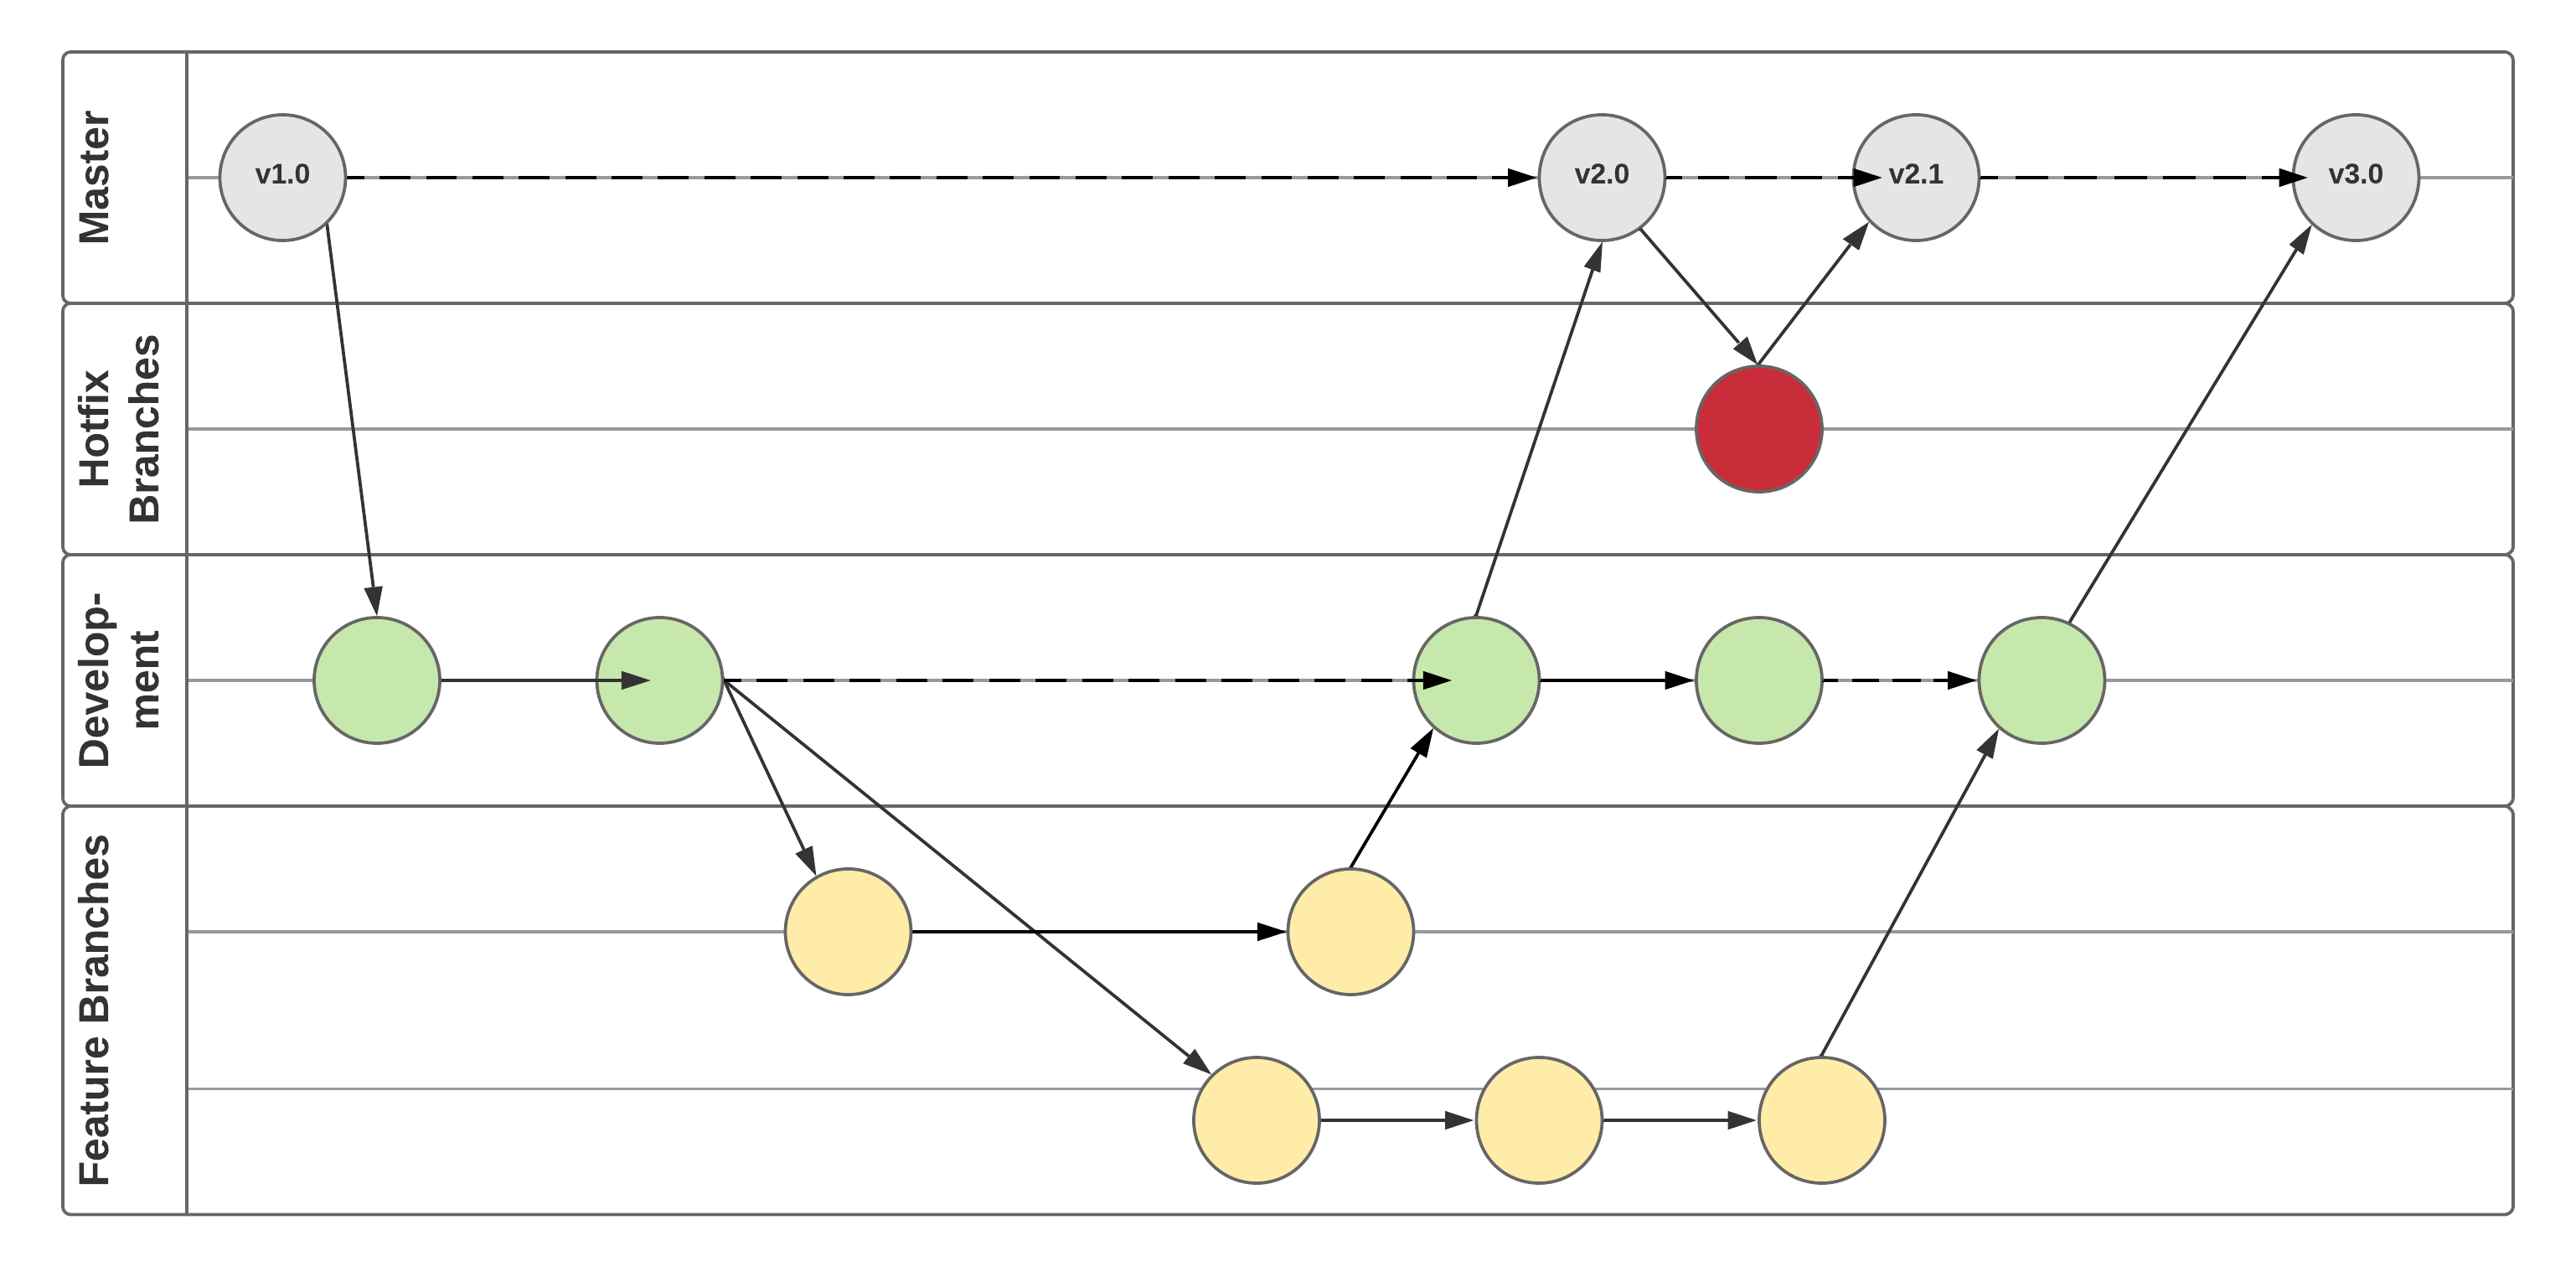
\includegraphics[width=6.25in,height=\textheight]{images/chapter2/git_flow.png}
\caption{Git workflow}\label{fig:git}
}
\end{figure}

There the project is split into several branches, which are represented
by a rectangular box. The circles represent single commits of new code.
Arrows are representing the push of a new version and dashed arrows are
representing the base version, on which the new commit was built and to
which it will be merged.

The most important branch is the master branch. On the master branch,
every finished version is pushed, and from this branch, it can be
released. The development branch is for ongoing changes. Small changes
can be done directly on the development branch. More significant
changes, like added features, should get their branch. Every developer
can create their branch for a new version so that the developers do not
interfere with each other. When all code changes are done, the new
version will be merged into the development branch. Sometimes some
conflicts in the code have to be fixed for a clean merge in case two
different commits changed the same code piece. As soon as the new
version is working on the development branch and everything is tested
and ready, it can be merged into the master branch, so that this new
version can be rolled out. In case an error occurs, it can be fixed in a
hotfix branch directly descending from the master branch.

Additionally, the application should be tested and verified
continuously. For that, the developer can run local unit tests to verify
their changes before integrating. Unit tests test a specific component
with defined input and output and checks if the calculated output is the
expected one. However, this does not verify that the integrated code
performs as designed.
{[}\protect\hyperlink{ref-AmazonDocumentation}{17}{]} A continuous
integration service like Jenkins can relieve the developer of this task
and automatically builds and runs unit tests on the newly committed and
integrated code. In doing so, it runs not only unit tests, but also
integration tests, which test the software as a whole. This process is
called \emph{continuous testing}.

Another critical point is to shorten the delivery cycles through an
end-to-end integration so that it needs less time to enroll a new
feature or similar. This method leads to quickly given feedback and
enables a faster reaction to this.
{[}\protect\hyperlink{ref-IBM2013}{16}{]} This approach takes place in
the \textbf{Deployment} stage of a product lifecycle and one of the root
capabilities of DevOps. It deals with the automation of the deployment
of the software to the different environments, which is called
\emph{continuous delivery}.

After the deployment follows the \textbf{Operation}. During this stage,
the performance of an application should be monitored, and feedback
should be collected. The results of this should be used to improve the
product as well as other products, that will be developed in the future.
For this, there are two practices defined - \emph{continuous monitoring}
and \emph{continuous feedback and optimization}.

\emph{Continuous monitoring} provides data and metrics to the
performance of an application as well as its running server, the
development cycle, the production, and other stakeholders.

\emph{Continuous feedback}, on the other hand, provides data coming
directly from the customer. This data includes the behavior of the users
as well as feedback provided by them.

Based on those retrieved data, businesses may adjust their plans and
priorities, improve the development cycle and features, and enhance the
environment in which the application is deployed in a more agile and
responsive way. The objective of this is to improve the product and
satisfy the users. Additionally, this knowledge should be used for new
products, that will be developed in the future.

\hypertarget{technologies}{%
\subsection{Technologies}\label{technologies}}

One technology to allow developers to follow above practices is
\textbf{Infrastructure as code}, which enables organizations to deploy
their environments faster and on a larger scale. This technology is
implemented with machine-readable definitions and configurations. Based
on them, the machine can provide the necessary environment automatically
to enable continuous delivery.

The most important technology for DevOps may be a \textbf{delivery
pipeline}. A delivery pipeline controls the product cycle of an
application from development to production. Typically there are four or
more stages - development, test, stage, and production. This can be seen
in figure \ref{fig:del_pipeline}.

\begin{figure}
\hypertarget{fig:del_pipeline}{%
\centering
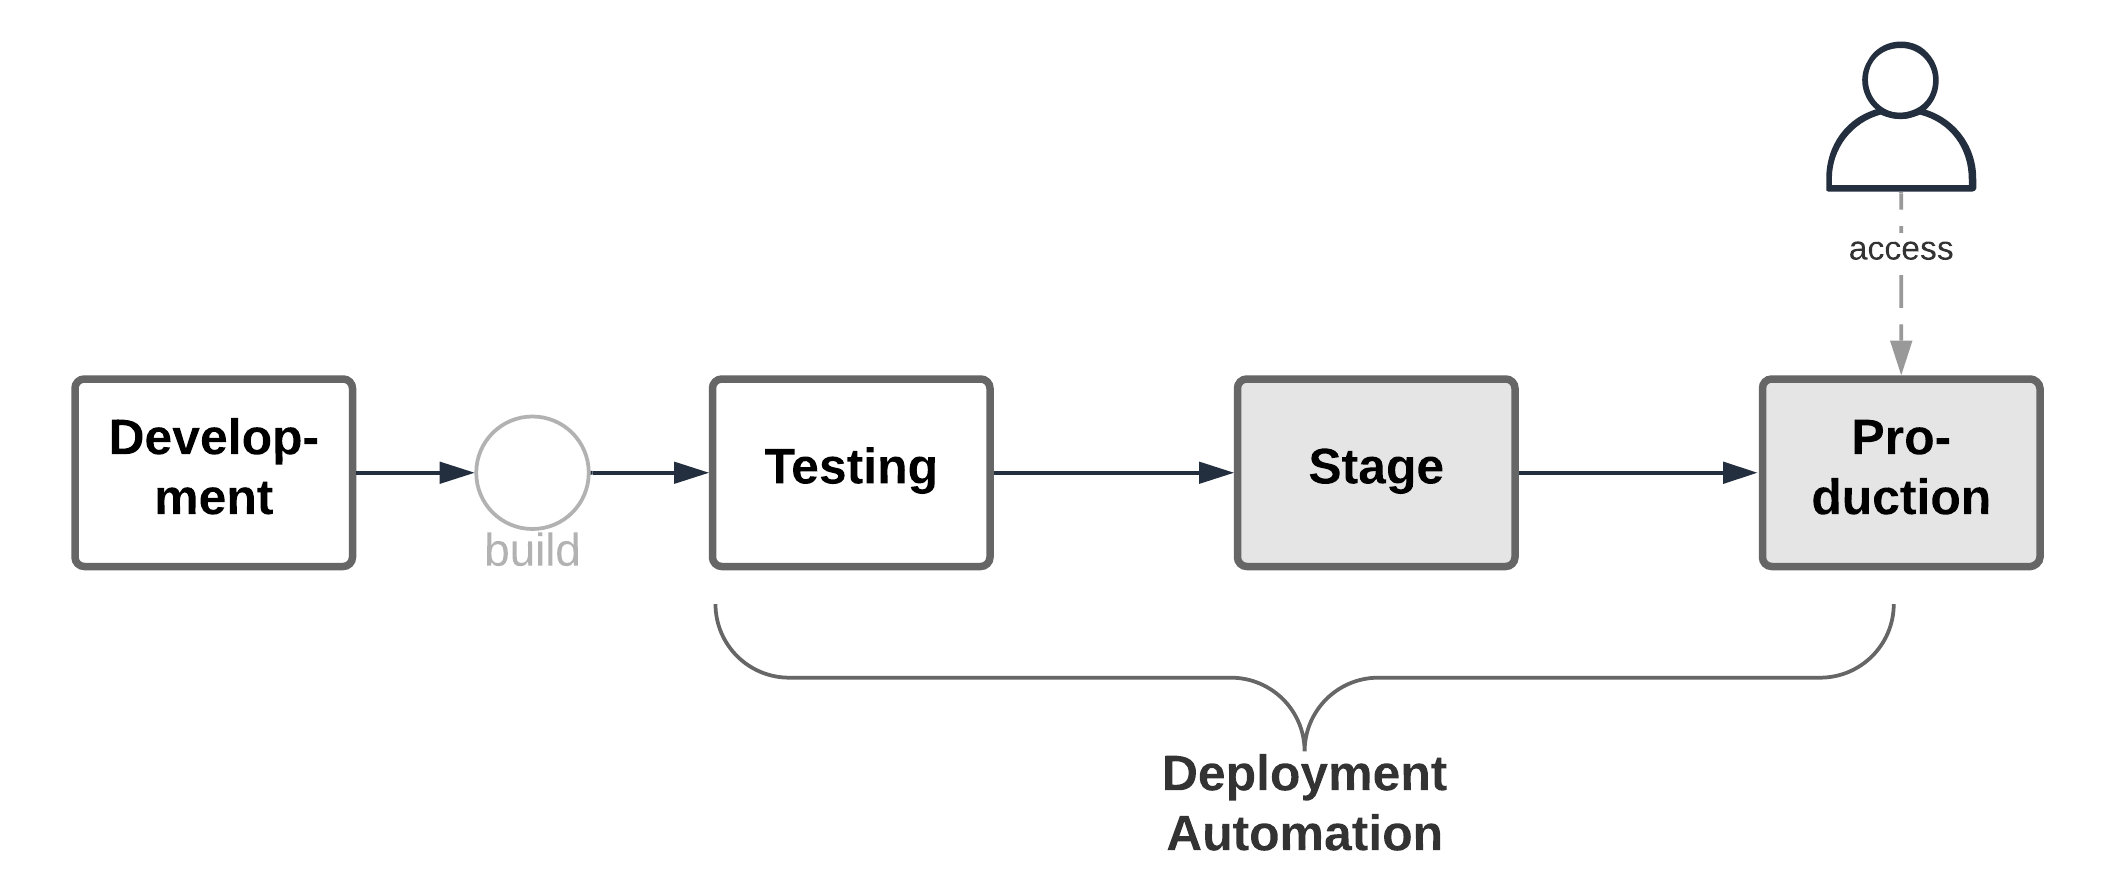
\includegraphics[width=4.16667in,height=\textheight]{images/chapter2/delivery_pipeline.png}
\caption{Delivery
pipeline{[}\protect\hyperlink{ref-Sharma2017}{15}{]}}\label{fig:del_pipeline}
}
\end{figure}

For every stage, there is usually one specific environment. Those are
represented as a box. The dark boxes represent a production like an
environment.

In the development environment, all the code updates are being done.
There are tools provided like \acs{IDE}s (\acl{IDE}) to write the code
as well as tools that enable collaborative development like source
control management or project planning.

Source control management is typically combined with version control.
This enables the developer also to store previous versions of his
application and reduces the risk of issues in new updates because it can
roll them back in case of an
error.{[}\protect\hyperlink{ref-TaliSoroker}{18}{]}

After the development, the delivery pipeline must care for the
application to be built.

Second, there is the testing environment, in which single components can
be tested. For that, it has to manage test data, scenarios, scripts, and
associated results. Similar to the development environment, it must not
look like the production environment.

The next one is the staging environment, in which the system can be
tested as a whole. The staging environment should be as much
production-like as possible so that as many as possible required
services, databases, and configurations can be connected and applied
without touching the production environment. The stage environment is
for testing the application before rolling out a major update.
{[}\protect\hyperlink{ref-MileciaMcG}{19}{]}{[}\protect\hyperlink{ref-Debbie}{20}{]}

The last one is the production environment, in which the application
will be running live and accessible for the users.

The delivery pipeline consists of all those stages and manages an
automated transition from one stage to the next one starting directly
after the development.

For this deployment automation tools are necessary, which perform the
deployments and track which version is deployed on which node. It also
manages changes that need to be performed for the middleware components
and configurations as well as database components or the environment.

Last, there should also be a tool for \textbf{release management}, which
provides a single collaboration portal for all stakeholders
participating in a project to plan and track the releases of an
application and its components across all stages.

With such technologies, most of the defined practices can be performed
with the help of accordingly educated people and well-thought-out
processes. However, DevOps is no static set of practices and tools, but
it changes with the changes in the world IT, such as Cloud or AI. In the
next chapters, these technologies will be reflected, and the impact
those have on DevOps will be analyzed.

\hypertarget{sec:ms12}{%
\section{Microservices and 12 factor apps}\label{sec:ms12}}

As described in chapter \ref{sec:cloud} Cloud opened new possibilities
of deploying and maintaining software. This eases the deployment itself
as well as rolling updates without any downtime. Additionally, it
enables high scalability as well as high availability.

One model of Cloud Computing is \acl{SaaS} (\acs{SaaS}). In this model,
an application is deployed on the provider's platform and is accessible
via the internet on demand. This way, the end-user can access the
software from anywhere anytime. In doing so, there is no need to deploy,
install, or maintain anything. The user has to pay-per-use, which means
that he only pays for the resources, which he has claimed.
{[}\protect\hyperlink{ref-Kumar2014}{21}{]}

However, the development and deployment of portable, resilient
applications that will thrive in Cloud environments are different from
traditional development. Because monolithic applications need to be
rebuilt entirely as soon as one component is being changed, the
development is unflexible. Additionally, the scaling of a single
component needs a scaling of the whole application. Both are
disadvantages which are opposed to the new possibilities a Cloud
deployment offers. The solution was to build those applications not as
one monolithic software but as a suit of services.

\hypertarget{microservice-architecture}{%
\subsection{Microservice Architecture}\label{microservice-architecture}}

For that, the term Microservice Architecture has sprung up over the last
few years. There is no unique definition for it, but when talking about
Microservice Architecture mostly, it is referred to Martin Fowler's
characteristics described in
{[}\protect\hyperlink{ref-MartinFowler}{22}{]}.

Following Fowler, the first characteristic is, that componentization is
realized via services. In monolithic software, different components are
linked together via libraries. Services on the other side are
out-of-process components. The communication is realized with web
service requests or remote procedure calls. The advantage of this
approach is that they are independently deployable, which is the reason
why this is the usual approach in Microservice Architecture.

A second characteristic is that Microservices are organized around
business capabilities. This means that the services take a broad-stack
implementation of software for that business era. This also leads to
cross-functional teams, which are working together on building the
Microservice.

Additionally, Microservices are handled as products instead of projects.
The difference is that while products are supported and owned by the
product team over its full lifetime, projects are not. They are
completed as soon as a specified set of functionalities is implemented.
After an operation team would support those projects. The approach to
treat Microservices as products has the advantage, that the development
team has full responsibility for it and are probably more interested in
a clean, well functioning long-term solution.

Another characteristic is the use of smart endpoints and dumb pipes,
which means that the services are as decoupled as possible. The only way
they stick together is that they receive requests of each other and
produce responses after applying the defined logic. This communication
is handled via simple \acs{REST}ish (\acl{REST} protocols.

Also, the governance of Microservices is usually decentralized so that
every service can be built on different technology platforms, and there
is a different approach to standards. This decentralization leads to a
more flexible environment.

The same applies to data management, which is decentralized as well.
Each service can manage its database, which avoids problems through
different conceptual models. While in centralized data management
changes are usually made via transactions, in a decentralized data
management system, there is transactionless coordination between the
services. This does not necessarily result in consistency, but this cost
is less than the cost, that would come up if a consistency would be
forced to Microservices by distributed transactions. Instead, the
problems this eventual consistency could cause are dealt with by
compensating operations.

The next characteristic is the automation of the infrastructure. This
includes automated testing and deployment. It is essential to test every
single Microservice intensively because the operational landscape for
each can be strikingly different. Also, the deployment could differ from
service to service.

Important for Microservices is that they are designed for failure. This
means that it detects failures quickly and automatically restore it in
case an error happens. This approach demands real-time monitoring. To
ensure this functionality, some companies are even executing tests in
production by purpose to observe the behavior of the system if one
service fails.o

The last characteristic defined by Fowler is the evolutionary design.
This design enables a more granular release planning because every
change can be handled as a single and only modified services needs to be
redeployed. These changes should not affect the communication with other
services, which is the reason why they should always be designed as
tolerant as possible.

The advantage of those Microservices for Cloud applications is mainly
caused by possibilities to treat every component as a single. This
improves the scalability, productivity, and the speed of the application
as well as the development. This is caused by the faster way of
developing such independent services. Additionally, it is easier to
maintain services instead of a monolith application, and it gives more
flexibility in technologies. Still, the development of Microservices
should follow some guidelines to support the concept of independently
managed and iterated services.

\hypertarget{factor-apps}{%
\subsection{12 factor apps}\label{factor-apps}}

One standard set of guidelines and best practices for the development of
Cloud-based software and especially Microservices are the 12 factors
drafted by developers at Heroku. These factors are

\begin{itemize}
\tightlist
\item
  Codebase - For every deployed service there should be precisely one
  codebase, for example, an IT repository
\item
  Dependency - Services should explicitly declare and isolate all
  dependencies
\item
  Config - Configurations for the deployments should be stored in the
  environment
\item
  Backing services - All backing services should be treated as attached
  resources
\item
  Build, release, run - The delivery pipeline should be strictly
  separated into building, releasing and running
\item
  Processes - Apps should be executed in one or more stateless processes
\item
  Port binding - Services should be exposed by listening on a specific
  port
\item
  Concurrency - Concurrency is achieved by horizontal scaling
\item
  Disposability - The objective should be a robust and resilient system
  with fast startup and graceful shutdown
\item
  Dev/prod parity - The development, staging, production and every other
  environment should be as similar as possible
\item
  Logs - Applications should produce logs as event streams
\item
  Admin processes - Admin tasks should be packaged alongside the
  application to ensure that it is run with the same environment
  {[}\protect\hyperlink{ref-Wiggins}{23}{]}
\end{itemize}

Following these guidelines, stable and performant Microservices can be
built. In the last years, some technologies have emerged as particularly
suitable for developing such services.

\hypertarget{container---docker}{%
\subsection{Container - Docker}\label{container---docker}}

One of them is containerization of applications. This can be understood
as a package for the isolation of application within a closed
environment, which provides everything the application needs. It is
comparable to a \acs{VM} (\acl{VM}), but much more light-weighted.
{[}\protect\hyperlink{ref-Jerry2015}{24}{]} This enables a light
deployment without unnecessary services or applications running in the
background, which leads to a very performant execution.

An industry-leading container engine technology is Docker. In figure
\ref{fig:docker_vm} the differences between a \acs{VM} and Docker can be
seen.

\begin{figure}
\hypertarget{fig:docker_vm}{%
\centering
\includegraphics[width=5.20833in,height=\textheight]{images/chapter2/docker_vm.png}
\caption{Comparison between Docker and
VM{[}\protect\hyperlink{ref-Mikesir87}{25}{]}}\label{fig:docker_vm}
}
\end{figure}

On the left side, the infrastructure of a VM can be seen, on the right
side, the infrastructure of a Docker container. Both need the
infrastructure of a physical device and its host operating system. On
top of a VM on this Host Operating System, there is a Hypervisor, and on
this Hypervisor several Guest OS can be running. On those again, the
apps itself can be executed, and the necessary libraries and binaries
are running in the background.

In case of a docker container, those binaries and libraries are directly
running inside of a container on the operating system. There is no need
for a hypervisor or a complete version of a Guest OS. This approach also
enables the app to be running on top of that. The containers are
isolated from each other in different namespaces and own network stacks.
This means that processes running within a container cannot see or
interact with processes of other containers, and they do not get
privileged access to sockets or interfaces of other containers.
{[}\protect\hyperlink{ref-DockerDocumentation}{26}{]}

Additionally, a Docker Daemon is running in another process. The Docker
Daemon has three main tasks - listening and processing API requests from
the Docker client to run Docker commands, managing Docker objects
(images, containers, volumes, and networks) and parsing Dockerfiles for
building Docker images. {[}\protect\hyperlink{ref-Lipke2017}{27}{]}

With this technology, several of the 12 factors described above are
fulfilled. One factor is the explicitly declared and isolated dependency
management. Within the Dockerfile, every dependency needs to be
explicitly declared to fulfill all the requirements of the application.
{[}\protect\hyperlink{ref-NoahZoschke}{28}{]}

Also, Docker containers cannot communicate with each other directly but
need to communicate externally over with backing services over the
network {[}\protect\hyperlink{ref-NoahZoschke}{28}{]}

Additionally, Docker containers are executed as stateless processes with
ephemeral storage only. {[}\protect\hyperlink{ref-NoahZoschke}{28}{]}

The development and production parity is given because containers
standardize the way of delivering applications as well as its
dependencies. {[}\protect\hyperlink{ref-NoahZoschke}{28}{]}

Even admin processes can be run as one-off processes inside the Docker
container through jumping inside the container and executing all
necessary commands.

Still, in a local environment, not each of the 12 factors is fulfilled.
Instead, an enabler is needed, which scalable and failure safe way to
deploy those containers.

\hypertarget{kubernetes-as-an-enabler}{%
\subsection{Kubernetes as an enabler}\label{kubernetes-as-an-enabler}}

Kubernetes can serve as such an enabler. It can host Microservices as
Docker containers and ensure all of the 12 factors to be met.

In general, Kubernetes enables an automated deployment, scaling, and
management of these containers within a cluster of nodes. Thereby a
cluster consists of at least one master node and any number of worker
nodes. Figure \ref{fig:kubernetes_services} shows the different services
owned by master and worker nodes.

\begin{figure}
\hypertarget{fig:kubernetes_services}{%
\centering
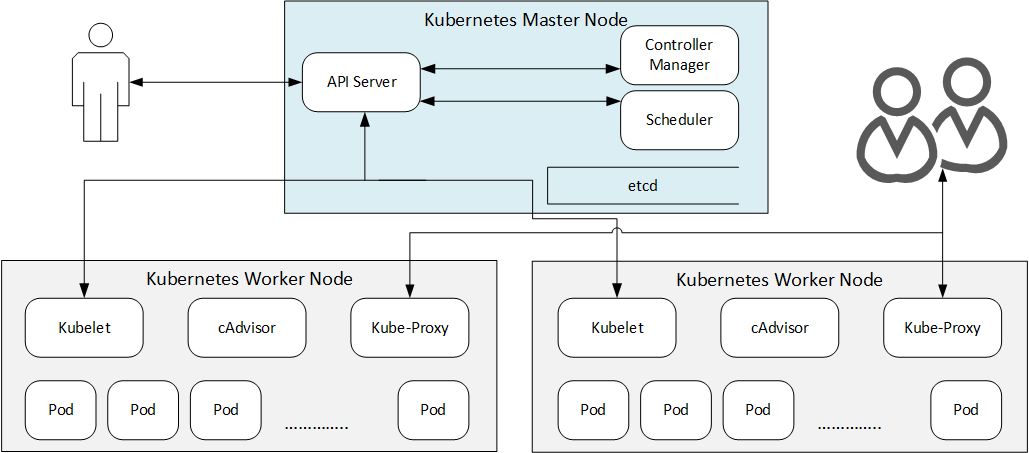
\includegraphics[width=5.20833in,height=\textheight]{images/chapter2/kubernetes.png}
\caption{Kubernetes service
allocation{[}\protect\hyperlink{ref-Fricke}{29}{]}}\label{fig:kubernetes_services}
}
\end{figure}

First, there are several pods on each worker node. Pods are the smallest
unit in Kubernetes. They contain one or more containers, which are
deployed together on the same host. There they can work together to
perform a set of tasks. {[}\protect\hyperlink{ref-CoreOS}{30}{]}

On the master node, there are an \acs{API} (\acl{API}) Server, a
Controller Manager, a Scheduler and a key-value store called etcd.
{[}\protect\hyperlink{ref-Fricke}{29}{]}{[}\protect\hyperlink{ref-JorgeAcetozi}{31}{]}

The API Server is for clients to run their requests against it. That
means the API Server is responsible for the communication between Master
and Worker nodes and for updating corresponding objects in the etcd.
{[}\protect\hyperlink{ref-Fricke}{29}{]}{[}\protect\hyperlink{ref-JorgeAcetozi}{31}{]}

The Controller Manager is a daemon, which embeds all of the Kubernetes
controllers. Examples for them are the Replication Controller or the
Endpoint Controller. Those controllers are watching the state of the
cluster through the API Server. Whenever a specific action happens, it
performs the necessary actions to hold the current state or to move the
cluster towards the desired state.
{[}\protect\hyperlink{ref-Fricke}{29}{]}{[}\protect\hyperlink{ref-JorgeAcetozi}{31}{]}

The scheduler manages the binding of pods to nodes. Therefore it watches
for new deployments as well as for old ones to create new pods if a new
deployment is created or recreating a pod whenever a pod gets destroyed.
The scheduler organizes the allocation of the pods within the cluster
based on available resources.
{[}\protect\hyperlink{ref-Fricke}{29}{]}{[}\protect\hyperlink{ref-JorgeAcetozi}{31}{]}

The etcd is a key-value store, which stores the configuration data and
the condition of the Kubernetes cluster.
{[}\protect\hyperlink{ref-Fricke}{29}{]}{[}\protect\hyperlink{ref-JorgeAcetozi}{31}{]}

The worker node consists of a Kubelet, a cAdvisor, a Kube-Proxy and - as
mentioned before - several Pods.

The Kubelet needs to be used if a new pod should be deployed. Then it
gets the action to create all needed containers. For that, it uses
Docker to create them. Afterward, it combines some containers into one
pod. Containers in one pod are always started and stopped together. This
pod will then be deployed on the node, on which the Kubelet is located.
{[}\protect\hyperlink{ref-Fricke}{29}{]}{[}\protect\hyperlink{ref-JorgeAcetozi}{31}{]}

The cAdvisor measures the usage of CPU-resources as well as demanded
memory on its node. That information is forwarded to the master node.
Based on those measurements, the scheduler allocates the pods within the
cluster to ensure the best possible allocation of resources.
{[}\protect\hyperlink{ref-Fricke}{29}{]}{[}\protect\hyperlink{ref-JorgeAcetozi}{31}{]}

The kube-proxy is a daemon that runs as a simple network proxy to
provide the possibility of communicating to that node within the
cluster.{[}\protect\hyperlink{ref-Fricke}{29}{]}{[}\protect\hyperlink{ref-JorgeAcetozi}{31}{]}

With this architecture, Kubernetes enables all the factors that are
missing in a local deployment of Docker containers.

First, the codebase of the deployment is given as YAML or JSON file and
the container in Dockerfile. This way, source control of all the
necessary code can be done using git, for example.
{[}\protect\hyperlink{ref-MichaelD.Elder}{32}{]}

Also, the dependencies for one Microservice can be checked easily with
the functions \emph{readinessProbe} and \emph{livenessProbe}. While the
\emph{readinessProbe} tests whether there are backing services, the
\emph{livenessProbe} tests if the backing services are all healthy. In
case of a missing or failed Microservice, the appropriate pod is
automatically restarted.
{[}\protect\hyperlink{ref-MichaelD.Elder}{32}{]}

For storing all the necessary configurations in the process environment
table, Kubernetes provides ConfigMaps. With these, the containers can
retrieve the config details at runtime.
{[}\protect\hyperlink{ref-MichaelD.Elder}{32}{]}

Stage separation is achieved through artifact management. Once the code
is committed, a build occurs, and the container image is built and
published to an image registry. These releases are then deployed across
multiple environments. {[}\protect\hyperlink{ref-MichaelD.Elder}{32}{]}

The port binding is guaranteed through Kubernetes services. These are
objects to declare the network endpoints of a service and resolve
endpoints of other services specified to a port of the cluster.
{[}\protect\hyperlink{ref-MichaelD.Elder}{32}{]}

The concurrency is a factor, which is handled especially extensively. It
allows the services to scale at runtime depending on the replica sets
defined in the declarative model. Also, Kubernetes has introduced
autoscaling based on compute resource thresholds.
{[}\protect\hyperlink{ref-MichaelD.Elder}{32}{]}

Also, disposability is fulfilled because every pod can be destroyed or
started quickly. Additionally, Kubernetes will automatically destroy
unhealthy pods. {[}\protect\hyperlink{ref-MichaelD.Elder}{32}{]}

Last, logs are written to \emph{stdout} and \emph{stderr} and can be
easily accessed. They are not stored and managed as internal files.
{[}\protect\hyperlink{ref-MichaelD.Elder}{32}{]}

This way, Docker and Kubernetes are fulfilling each of the 12-factors,
which shows that it is an excellent way to provide Microservices. This
is the reason why many big companies decided to use Kubernetes as an
enabler for big platforms like Google Cloud to give just one example.

\hypertarget{sec:ml}{%
\section{Machine Learning}\label{sec:ml}}

Another eminent movement in IT is Machine Learning, which helped AI to a
new hype and opened several new possibilities and improvements to
software development. Because of the exponential growth of computation
power and data, Machine Learning has become one of the most important
tools when it comes to Artifical Intelligence.

The advantage of Machine Learning compared to traditional software
development is, that it eliminates the need to write the code by
oneself. Instead, the developer enters some input data to the Machine
Learning system. This system then figures out mathematical functions,
which describes the given collection of data points best. The process of
finding these function is called Machine Learning, and the resulting
function is mostly referred to as model.

This results in a system, which continuously improves the more data it
is fed with because this leads to a more accurate function. Based on
this assumption, Tom Mitchell defined Machine Learning in 1997 as
follows:

\newtheorem{definition}{Definition}

\begin{definition}

A computer program is said to learn from experience E with respect to some class of tasks T and performance measure P, if its performance at task in T, as measured by P, improves with experience E. 

\end{definition}

{[}\protect\hyperlink{ref-Mitchell:1997:ML:541177}{33}{]}

This definition means that a computer program learns if it is improving
its performance at some task through experience. This experience could
be input data like pictures of trees, with which it gets trained with
the task to identify those trees on that picture.

\hypertarget{tasks}{%
\subsection{Tasks}\label{tasks}}

For fulfilling such a task, it is necessary to define this task before.
This definition is oriented to the book \enquote{Deep Learning} by Ian
Goodfellow, Yoshua Bengio, and Aaron Courville.
{[}\protect\hyperlink{ref-Goodfellow-et-al-2016}{34}{]}

In general, tasks are described in terms of how the Machine Learning
system should process an example. An example is a collection of
quantitative measurements, called features. This set can be written as a
vector \(x \in \mathbb{R}^n\) with each \(x_i\) being one of the
features.

The most important and most common tasks in computer science are

\begin{itemize}
\tightlist
\item
  Classification
\item
  Regression
\item
  Structured Output
\item
  Anomaly detection
\item
  Missing Values
\end{itemize}

In \emph{classification}, the objective is to figure out the category of
an example out of a data set by given features. Mathematically this can
be described as a function, that takes an example with all its features.
Then it assigns a category out of an appropriate set. This set of
categories is limited to k so that it can be described as \({1,...,k}\).
This function can be represented as follows:

\begin{equation}\label{eq:classification }

f: \mathbb{R}^n \rightarrow {1, .., k}

\end{equation}

An example of this is character recognition. It gets an image of a
character as input. Then, the task is to assign this image to one
element of the set of characters.

The objective of a \emph{Regression} is to predict a numeric value by
given input data. This can be formulated as

\begin{equation}\label{eq:regression }

f: \mathbb{R}^n \rightarrow \mathbb{R}

\end{equation}

When the function that has to be learned is of the form \(y=f(x)\) with
\(y \in \mathbb{R}\) and \(x \in \mathbb{R}^n\) then \(x\) should be a
set of independent variables and \(y\) should be a dependent variable on
\(x\).

An example of a Regression is a prediction of the costs for a new
apartment based on features like size, location, and the number of
rooms.

\emph{Structured Output} tasks ask a learning algorithm to figure out
the probability distribution that has produced the data set. This value
is then used to give an estimation of the relationship between single
examples from the data set.i

A well-known example of this is to recommend products based on
previously bought products. For that, the learning algorithm figures out
the similarity between the products and recommends those with the
highest consistency.

\emph{Anomaly detection} works similar to Structured Output, but instead
of looking for elements with a great relationship, it uses the
probability distribution to check for irregularities within the dataset.

This is an excellent way to anticipate a fraud in a banking account
through checking every transaction and hold back those, which are
looking too irregular.

For \emph{Missing Values}, the probability distribution is used to infer
what value should most likely be set at a specific position of a given,
incomplete set of examples. This means that a set \(x \in \mathbb{R}\)
with some \(x_i\) missing. The objective is to figure out the best
values for these missing entries.

An example of this is to predict a logical sequence of numbers without
the need to know the exact formula of the sequence.

\hypertarget{training-approaches}{%
\subsection{\texorpdfstring{\textbf{Training
approaches}}{Training approaches}}\label{training-approaches}}

As mentioned above, in Machine Learning, all those tasks are not solved
by explicitly coding algorithms and formulas, but by training a system
with given input data. For training those systems, different approaches
are existing, each used for different requirements. This chapter will
also be based on the book \enquote{Deep Learning}.
{[}\protect\hyperlink{ref-Goodfellow-et-al-2016}{34}{]}

One of the viable approaches is called supervised learning. Supervised
learning requires an additional value for each example representing the
optimal solution for it. Formally the data set can be described as
\(\mathbb{D} \in 2^{\mathbb{R}^n}\). For every example vector
\(x \in \mathbb{D}\) there exists a \(y \in \mathbb{R}\) such that
\(y=f(x)\) with \(f:\mathbb{R}^n \rightarrow \mathbb{R}\) being the
function that describes the task to be learned. This additional feature
is mostly referred to as label or target. Usually, the tasks are
accomplished by approximating the conditional probability distribution
\(p(x|y)\).

Supervised learning algorithms are often used for classification or
regression tasks.

Unsupervised learning, on the other hand, does not have any additional
features but has to work with the pure, raw data set. Usually, the data
points have many features, and the task is to figure out some useful
property about the relationship between these data points. This is
usually done by using the probability distribution function \(p(x)\) of
the data set.

Semi-supervised learning uses both - unlabeled examples as well as
labeled examples - to predict the outcome. This approach facilitates the
task for the developer, because not every data point has to be labeled,
but decreases the size of labeled examples, which could worsen the
resulting model.

Common tasks for unsupervised learning are clustering or anomaly
detection.

In figure \ref{fig:training_comparison}, a comparison between supervised
and unsupervised data sets used for clustering and classification can be
seen. The data shown is not of a particular use case and just for
demonstration purposes. In both representations, the examples of the
data set have only two features, one corresponding to the x-axis and the
other on the y-axis. The task is to identify clusters in the data.

\begin{figure}
\hypertarget{fig:training_comparison}{%
\centering
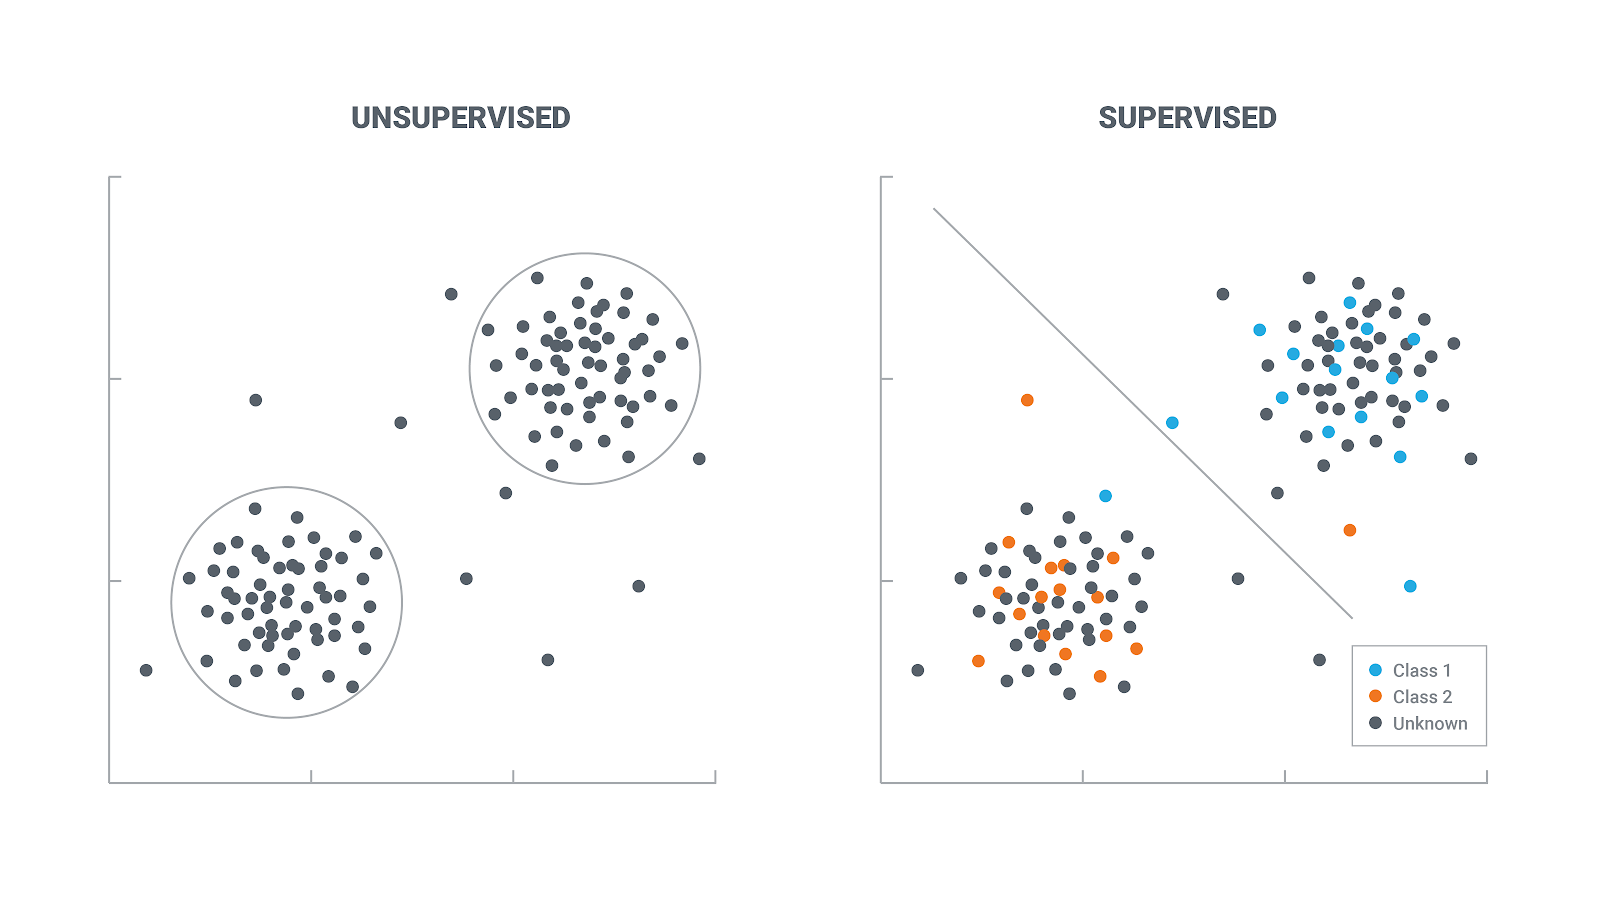
\includegraphics[width=6.25in,height=\textheight]{images/chapter2/training_comparison.png}
\caption{Comparison of unsupervised and semi supervised data sets used
for
clustering{[}\protect\hyperlink{ref-AmnahKhatun}{35}{]}}\label{fig:training_comparison}
}
\end{figure}

The difference is that some of the data points of the second data set
are labeled with either \enquote{Class 1} or \enquote{Class 2}. In the
figure, this can be seen by the coloration of the data points. Even
though in this example there are only some data points labeled, which is
the reason why the applied learning approach is called semi-supervised
learning, it is still functioning as an example for supervised learning
and demonstrates the differences to the unsupervised model.

The missing labels force the first example to only use the features
\(x\) and \(y\) and look for similarities to determine its association
with a group. In the second examples, the algorithm can use the labels
as well to determine a function, which assigns a class to every data
point.

In the figure on the left side, two clusters can be seen, which are
circled in a group. On the right side, there is a line, which marks the
function splitting the dataset into two groups. It is noticeable that
the first approach leads to some examples, which cannot be assigned to
either of the classes.

Additionally, there is another approach called reinforcement learning.
In reinforcement learning, a model is built and then iteratively
improved by taking in further examples. For that, it needs to get some
feedback on how good the built model is. For example, this can be a
reward or punishment function.

\hypertarget{sec:nnmodels}{%
\subsection{Models}\label{sec:nnmodels}}

With the approaches mentioned above the objective is to create and train
a model, with which the tasks can be fulfilled. In modern Machine
Learning, the most important type of such models are \acl{ANN}s
(\acs{ANN}s).

Neural Networks are inspired by biological neural networks like animal
brains. According to that, \acs{ANN}s are based on a collection of nodes
called artificial neurons. Each neuron gets one or more input values and
one output value. To generate the output value, the neuron does some
mathematical computations with the input values.
{[}\protect\hyperlink{ref-Stroetmann2018}{36}{]}

A network of such neurons usually persists out of at least three layers.
The first layer is the input layer of the data, with which the neural
network should be fed. Those values are then sent to every neuron of the
hidden layer. Those are doing the necessary calculations described below
and send their output to the output layer.
{[}\protect\hyperlink{ref-Stroetmann2018}{36}{]} This can be seen in
figure \ref{fig:neural_net}.

\begin{figure}
\hypertarget{fig:neural_net}{%
\centering
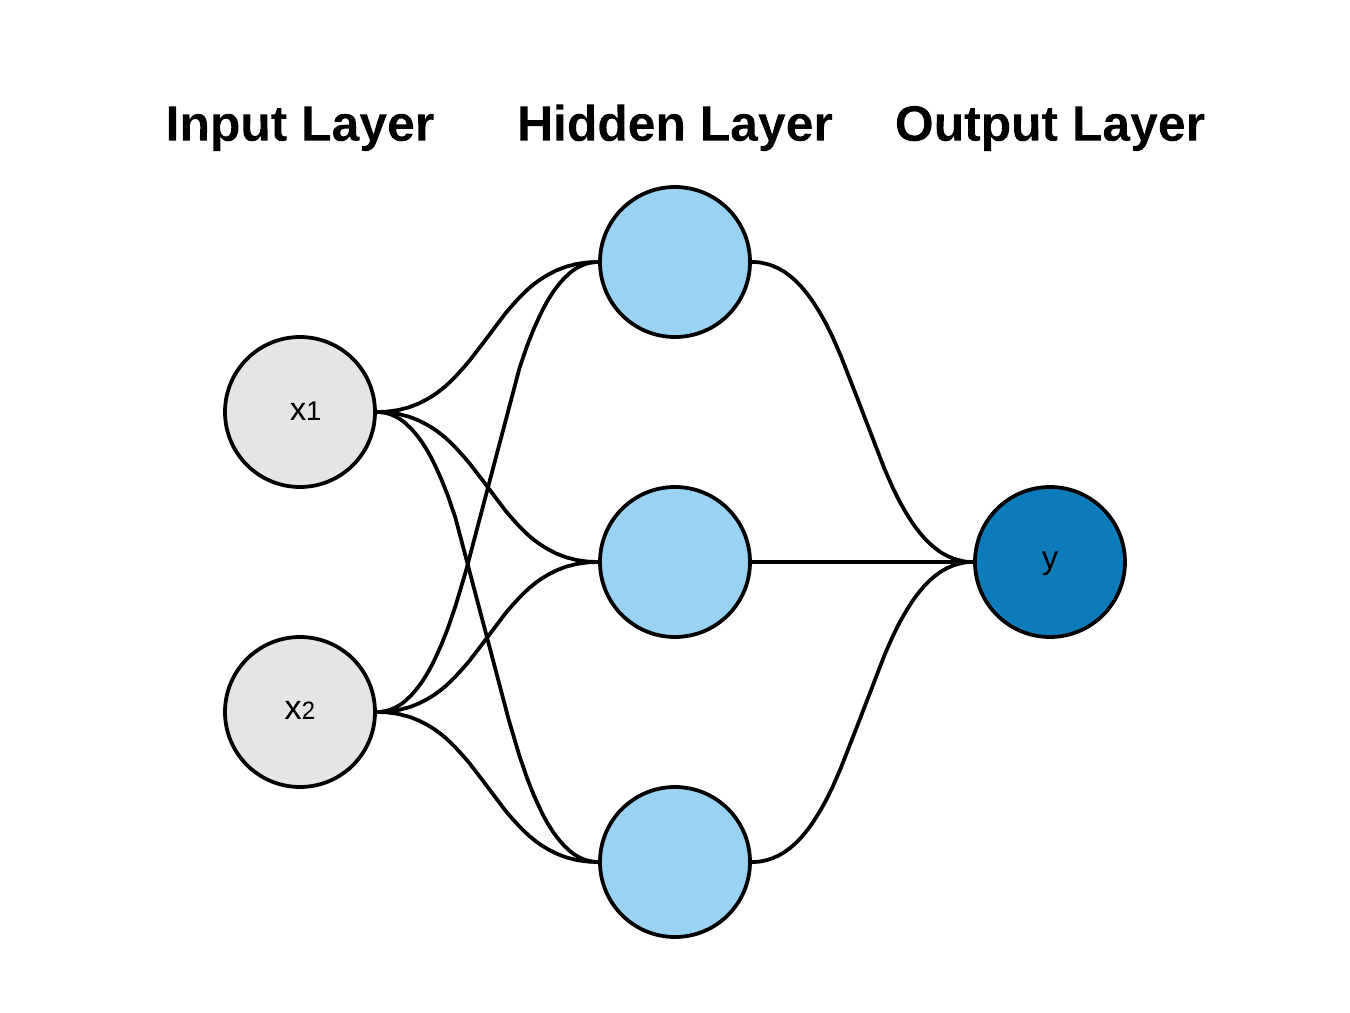
\includegraphics[width=4.16667in,height=\textheight]{images/chapter2/neural_net.png}
\caption{Simple neural network}\label{fig:neural_net}
}
\end{figure}

On the hidden layer the neurons are combining the inputs and calculating
a new value with them. For that three parameters need to be given to
generate the output \(y\) with the input vector \(x\):

\begin{itemize}
\tightlist
\item
  A weight vector \(w\)
\item
  A bias \(b\)
\item
  An activation function \(f(x)\)
  {[}\protect\hyperlink{ref-VictorZhou}{37}{]}
\end{itemize}

The weight vector is used to weight the different inputs. This means,
that each input is multiblied by a weight as can be seen in equation
{[}\protect\hyperlink{ref-VictorZhou}{37}{]} \ref{eq:weight}

\begin{equation}

x_1 \rightarrow x_1 * w_1

\end{equation}

After that, all the weighted inputs are added together. Additionally the
bias \(b\) is added to this formula:
{[}\protect\hyperlink{ref-VictorZhou}{37}{]}

\begin{equation}

(x_1 * w_1) + (x_2 * w_2) + b

\end{equation}

Finally, the activation function is being used to generate the output.
For that it takes the sum calculated in the above equation as input:
{[}\protect\hyperlink{ref-VictorZhou}{37}{]}

\begin{equation}

y = f((x_1 * w_1) + (x_2 * w_2) + b)

\end{equation}

A typical activation function is the sigmoid function, which outputs
numbers in the range (0,1). The higher the input, the closer the result
gets to 1. The lower the input, the closer it gets to 0. The sigmoid
function can be seen in \ref{eq:sigmoid}
{[}\protect\hyperlink{ref-VictorZhou}{37}{]}

\begin{equation}

y = \frac{1}{1 + e^{-x}}

\end{equation}

In figure \ref{fig:neuron} this whole process, that happens within the
artificial neuron, can be seen in a simplified way. It takes the inputs
\(x_1\) and \(x_2\), multiplies them with their belonging weights, sums
up the results and adds a bias. Finally, it takes the result of this
calculation as input for the activation function. The result of this is
the output \(y\). {[}\protect\hyperlink{ref-VictorZhou}{37}{]}

\begin{figure}
\hypertarget{fig:neuron}{%
\centering
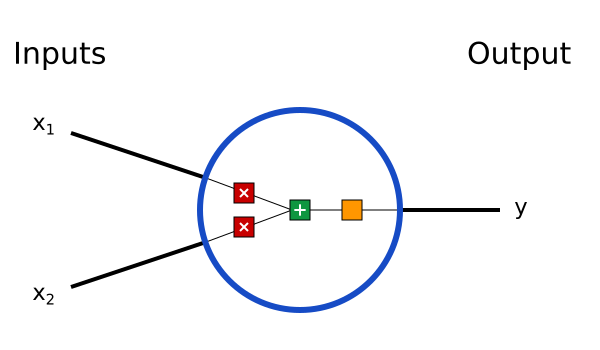
\includegraphics[width=4.16667in,height=\textheight]{images/chapter2/neuron.png}
\caption{2 input
Neuron{[}\protect\hyperlink{ref-VictorZhou}{37}{]}}\label{fig:neuron}
}
\end{figure}

A neural network can consist of more than one hidden layer. In that
case, these networks are called deep neural network. In figure
\ref{fig:deep_nn} such a deep neural network with three hidden layers
and two output values can be seen.
{[}\protect\hyperlink{ref-Stroetmann2018}{36}{]}

\begin{figure}
\hypertarget{fig:deep_nn}{%
\centering
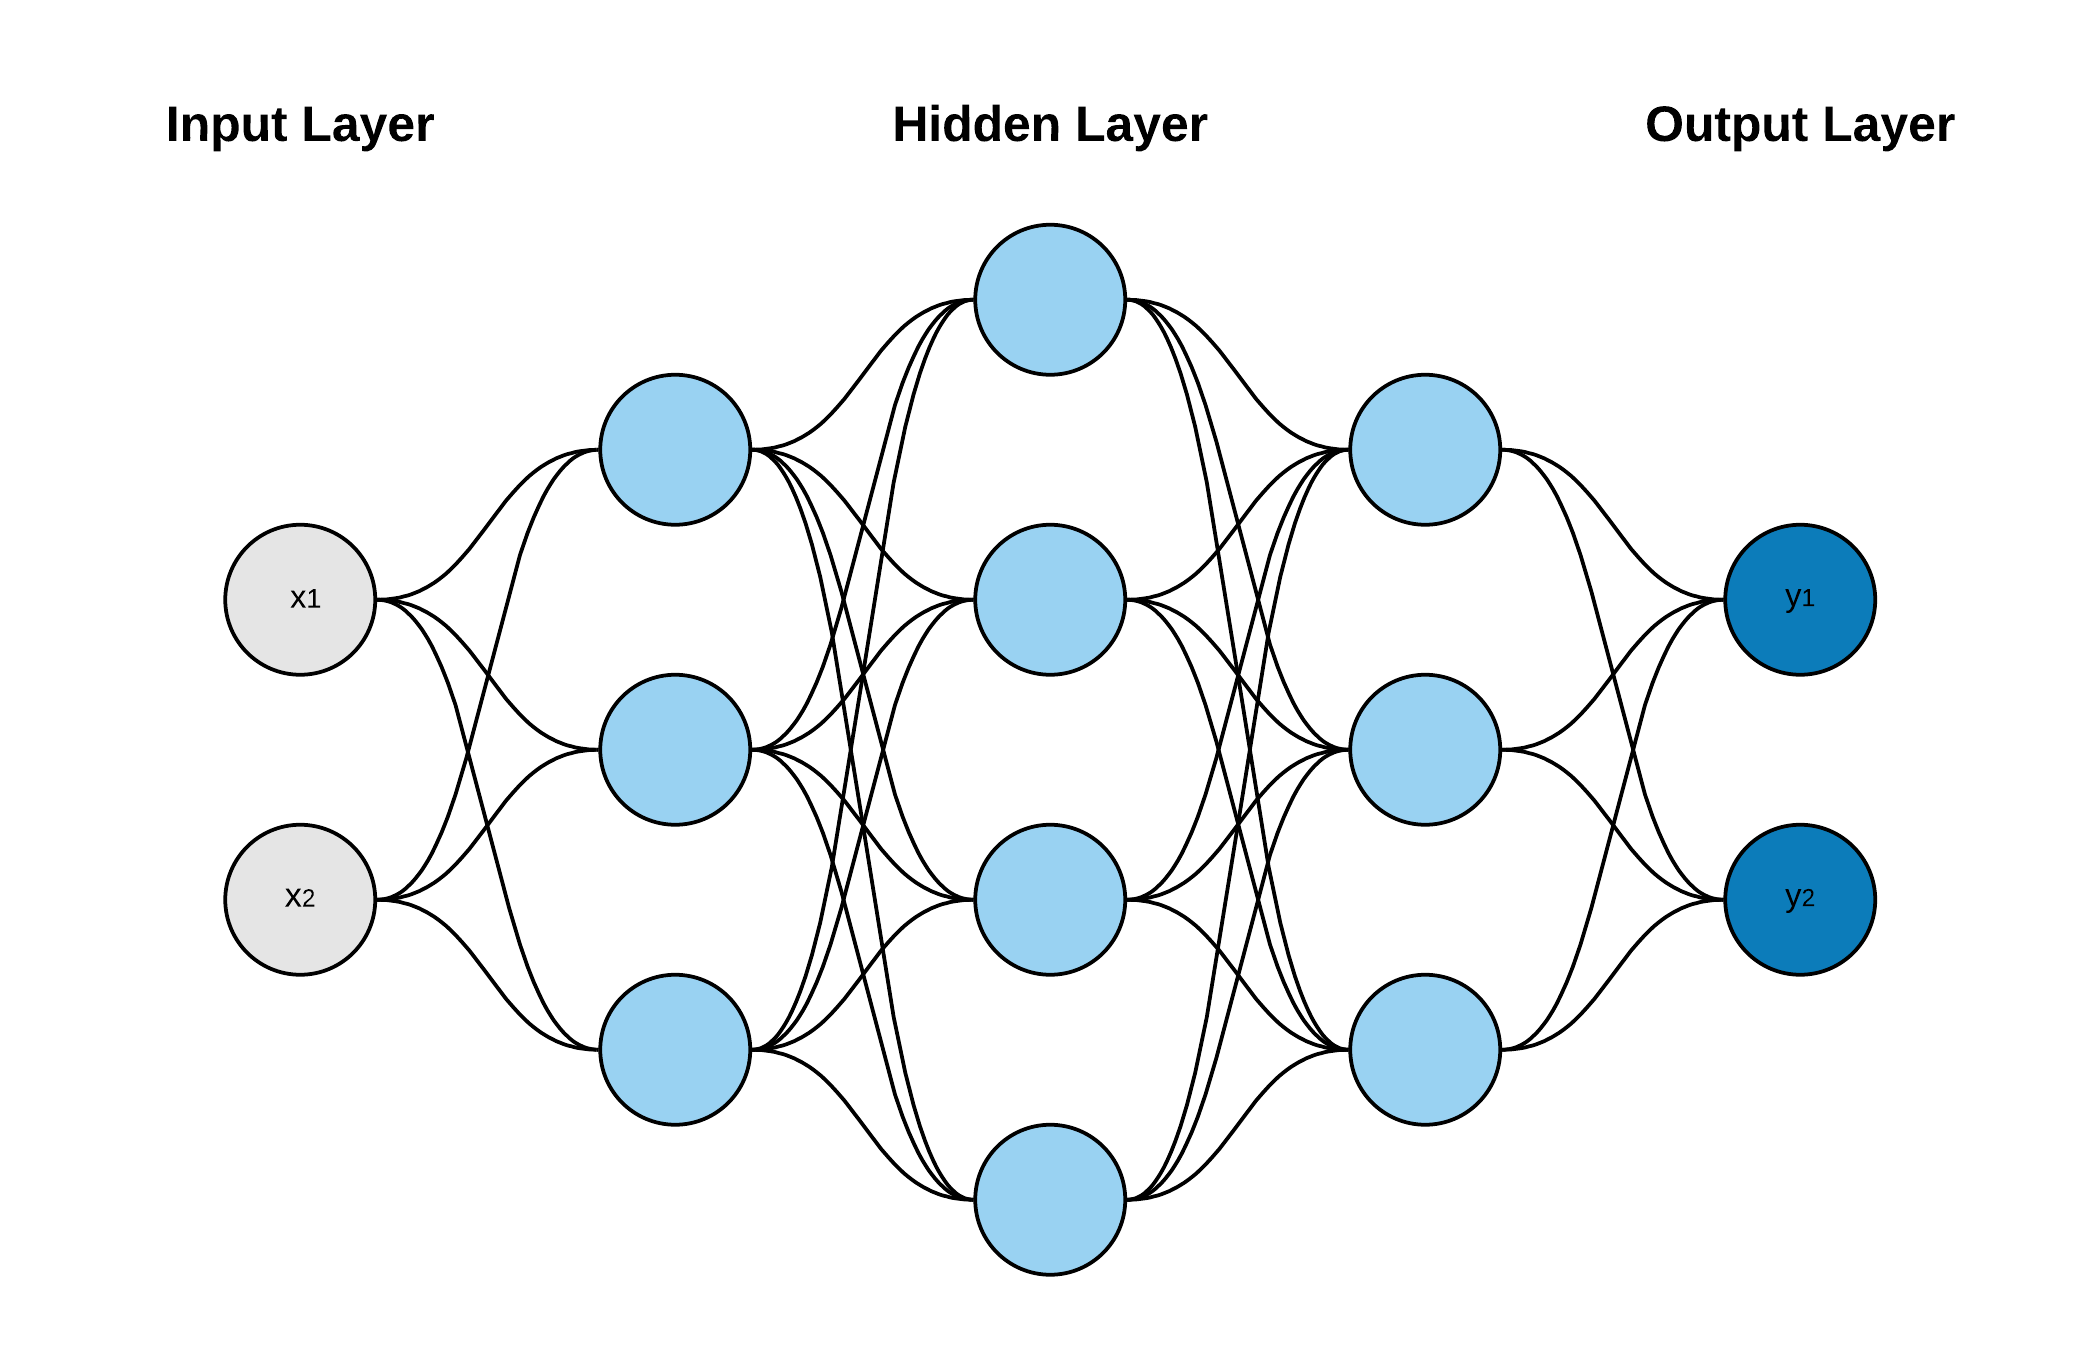
\includegraphics[width=5.20833in,height=\textheight]{images/chapter2/deep_neural_net.png}
\caption{Deep neural network with 3 hidden layers}\label{fig:deep_nn}
}
\end{figure}

When training a network, the objective is minimizing the loss function.
The loss function is a function, which provides information about how
good the neural network is. One common loss function is the Mean Squared
Error: {[}\protect\hyperlink{ref-VictorZhou}{37}{]}

\begin{equation}

MSE = \frac{1}{n}\sum*{i=1}^{n}{(y*{true}-y_{pred})^2}

\end{equation}

With \(n\) as the number of samples, \(y_{true}\) as the true value of
the variable and \(y_{pred}\) as the predicted value of it. To minimize
this loss, the neural network uses the partial derivative to change the
weights and biases accordingly. This is done over and over again for
every sample until the network is well-trained with the given inputs.

Still, the developer does not only have to give some input data, train
the neural network, and think all his work is done. Instead, other
challenges have to be faced like preparing the data, choosing the right
parameters and amount of input data to get the best results and avoid
problems like over- or underfitting the network. Overfitting means that
a network is trained with too many irrelevant features, called noise.
Overfitting leads to a perfectly working system for the known data,
which, on the other hand, does not work at all for unknown data, because
it is too specialized on the data on which it was trained. Underfitting,
on the other hand, occurs if the neural network was informed by too few
features or regularized too much, which prevents the neural network from
learning from the dataset. How the developer handles these difficulties
and what the necessary steps are in this new kind of development will be
described in chapter \ref{sec:aicycle}.
{[}\protect\hyperlink{ref-Goodfellow-et-al-2016}{34}{]}

\hypertarget{sec:aicycle}{%
\section{Artificial Intelligence lifecycle}\label{sec:aicycle}}

The new possibilities opened by Machine Learning, as described in
chapter \ref{sec:ml} force developers to change their development
lifecycle in a drastic way if they want to develop a Machine Learning
based Artificial Intelligence. This lifecycle will be described and
explained in the following chapter.

Important to mention is, that instead of code the developers have to
produce for a specified objective, in Machine Learning the developers
get some data as input and must train a model with this data to meet the
objective. To simplify the process described in this chapter an example
data set will be given and in the process of explaining the single steps
this data will be used to exemplify these. This dataset can be seen
below.

\begin{table}[htb]

\centering

\small

\rowcolors{2}{gray!25}{white}

\caption{Example dataset to predict the price of real estate}

\begin{tabular}{ c | c | c | c | c | c | c  }

\rowcolor{gray!50}

\textbf{square meters} &\textbf{year built} &\textbf{year bought} &\textbf{age of buyer} &\textbf{type} &\textbf{# of rooms} &\textbf{price} \ \hline

50 & 2000 & 2005  & 33 & Appartm. & 3 & 250.000€ \

20 &  & 2010 & 26 & Appartm. & 1 & 100.000€ \

160 & 2004 & 2004 & 38 & House & 5 & 500.000€ \

300 & 2010 & 2016 & 41 & House & 7 & 680.000€ \

80 & 2018 & 2018 & 29 & Appartm. & 3 & 290.000€ \

48 & 1999 & 2008 & 24 & Appartm. & & 220.000€ 

\end{tabular}

\end{table}

With this data the developer has to go through several steps to build a
useful system based on them. These steps are defined in an open standard
process model called \acl{CRISP-DM} or \acs{CRISP-DM}. This model can be
seen in figure \ref{fig:crisp_dm}.

\begin{figure}
\hypertarget{fig:crisp_dm}{%
\centering
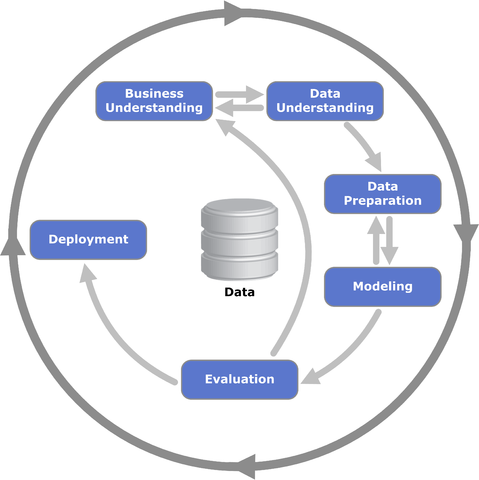
\includegraphics[width=4.16667in,height=\textheight]{images/chapter2/crisp_dm.png}
\caption{CRISP-DM
standard{[}\protect\hyperlink{ref-WolfRiepl}{38}{]}}\label{fig:crisp_dm}
}
\end{figure}

Following this standard model, the first step is Business Understanding.
During this step, the project team has to determine overall goals and
tasks for what to do with these data. For that, the team has to access
the situation, which means that the team has to include possible risks,
costs, benefits, and requirements for every possible objective in their
evaluation process. After the overall objective is defined, this can be
partitioned into several data mining goals what to do specifically with
this data. Also, success criteria should be defined, and a project plan
should be established, which will be followed in the next steps.
{[}\protect\hyperlink{ref-Wirth2000}{39}{]}

For the example above, such an objective could be to predict the price
of real estate by the given features. The criteria could be, that in
90\% of the tested data after the creation of the model, the predicted
price should lie in between a range of 10\% of the original price.

Next, the data need to be understood. For that, first, as much data as
possible should be collected and analyzed to get a first insight. This
data should then be evaluated by its quality to estimate the necessary
effort to prepare and clean the data for building a model. Also,
possible problems should be detected early to fix them as soon as
possible. {[}\protect\hyperlink{ref-Wirth2000}{39}{]}

In the example, there are far too little data for a real model, and much
more would be needed in a real project. However, even in this small
dataset, some problems can be detected. The first one is the missing
entry for the second object in the column \enquote{year built} as well
as for the last object in the column \enquote{\# of rooms}. Also, the
type of estate is categorical instead of numerical, which could cause
problems when training the model.

The next step is probably the one that needs the most effort of the
developer - data preparation. First, the project team needs to select
the data, which it will use for building the model. Then the data need
to be preprocessed. {[}\protect\hyperlink{ref-Wirth2000}{39}{]}

This preprocessing step includes detecting and removing noisy and
redundant data. Noisy data means data that are irrelevant to the chosen
business objective. In the given example, the age of the buyer is
unnecessary information because it does not change the price of the
estate. This circumstance is why this column can be removed. Also,
wrongly labeled data should be removed.

Additionally, in the preprocessing step, unbalanced datasets should be
balanced. This means that if one specific class of data is
overrepresented and another one underrepresented, the dataset should be
balanced so that the distribution of the different data classes are
representative. In the example, apartments could be overrepresented,
because there are twice as many apartments in the selected data than
houses. The solution would be to add some more houses in the dataset or
remove some apartments.

Last missing values have to be handled because null values could
negatively influence the model. A better way would be to fill the
missing cells with average values for this type of data. However, to
choose the average value is not always the right way - it could be
better to choose the minimum, for example. To decide the method of
handling missing values is one challenging task for the developer.
{[}\protect\hyperlink{ref-article}{40}{]}

After the preprocessing, the dataset could be improved by feature
engineering. The objective of this task is to improve the features such
that the model better understand the coherences and improves its
production function. {[}\protect\hyperlink{ref-article}{40}{]} For
example, new features could be created based on the knowledge of the
data. A condition for that is to have an excellent understanding of the
data. In the example above the developers could combine the column
\enquote{year built} and \enquote{year bought} to \enquote{age at date
of purchase} with a simple subtraction, which could give an essential
insight of the price. Another meaningful feature could be some relation
between the size of the real estate and the number of rooms.

Additionally, there can be features in a dataset that are not numerical
but categorical. This data need to be encoded before training the model.
The encoding technique depends on the context of the categorical data.
One simple technique is label encoding, with which for every different
category tha column gets a different number. For example every
\enquote{Appartment} gets a 1 and every \enquote{House} a 2 in the
\enquote{type} column. However, this could cause trouble, because the
learning algorithm could interprete the numbers as sequence. That's why
another technique is One-Hot-Encoding. In this technique every possible
category gets an own column and for every entry in the dataset the value
is set to either 1 or 0 for all of the columns. In the example this
would mean, that the column \enquote{type} would be replaced with the
columns \enquote{appartment} and \enquote{house}. For every appartment
the column \enquote{appartment} would then be set to 1 and the column
\enquote{house} to 0. For every house it would be exactly the other way
round.{[}\protect\hyperlink{ref-SunnySrinidhi}{41}{]}

In the next step all collected and cleaned data should be integrated and
merged. After that the feature values should be normalized, because
there is usually a significant difference between the minimum and the
maximum value of a feature. To increase the performance of a model it
could be helpful to scale the values down to, for exaple, a range from 0
to 1. {[}\protect\hyperlink{ref-article}{40}{]}

In the end the example above could look like this:

\begin{table}[htb]

\centering

\small

\rowcolors{2}{gray!25}{white}

\caption{Example dataset to predict the price of real estate}

\begin{tabular}{ c | c | c | c | c | c | c  }

\rowcolor{gray!50}

\textbf{square meters} &\textbf{year built} &\textbf{year bought} &\textbf{age at purchause} &\textbf{type} &\textbf{# of rooms} &\textbf{price} \ \hline

0.11 & 0.05 & 0.07  & 0.56 & 0.00 & 0.33 & 0.26 \

0.00 & 0.50 & 0.43 & 0.22 & 0.00 & 0.00 & 0.00 \

0.50 & 0.26 & 0.00 & 0.00 & 1.00 & 0.67 & 0.69 \

1.00 & 0.58 & 0.86 & 0.67 & 1.00 & 1.00 & 1.00 \

0.21 & 1.00 & 1.00 & 0.00 & 0.00 & 0.33 & 0.33 \

0.10 & 0.00 & 0.29 & 1.00 & 0.00 & 0.50 & 0.21

\end{tabular}

\end{table}

This data set has then to be splitted into three different sets -
training, validation and testing. This is done to ensure that the model
does not overfit to the training data. The model will be trained with
the training set. Then the hyperparameters, which are used to improve
the model with some different parameters dependent on the used model,
are tuned with the help of the validation set. The test set is used to
test the models actual performance at the end.

After this, the next step is modeling. For this, first, a training
technique, as well as a basic model, has to be selected. Usually,
different models are tested several times, so that the best model can be
chosen in the end. This model will then be used to train it with the
training set. As already mentioned above the hyperparameters are then
tuned with the help of the validation set. This prevents, for example,
over- and underfitting the model with the training data.
{[}\protect\hyperlink{ref-Wirth2000}{39}{]}

Then the model has to be evaluated with the test set. Also, the whole
process needs to be reviewed and improved if possible. Dependent on the
resulting model and the satisfaction of all stakeholders, the steps can
be repeated starting from the Business Understanding with deeper
knowledge. This is how a model can be continuously improved until all
stakeholders are satisfied by tuning the hyperparameters, choosing
different models or improved data and features, or applying different
training methods. {[}\protect\hyperlink{ref-Wirth2000}{39}{]}

\begin{figure}
\hypertarget{fig:ml_cycle}{%
\centering
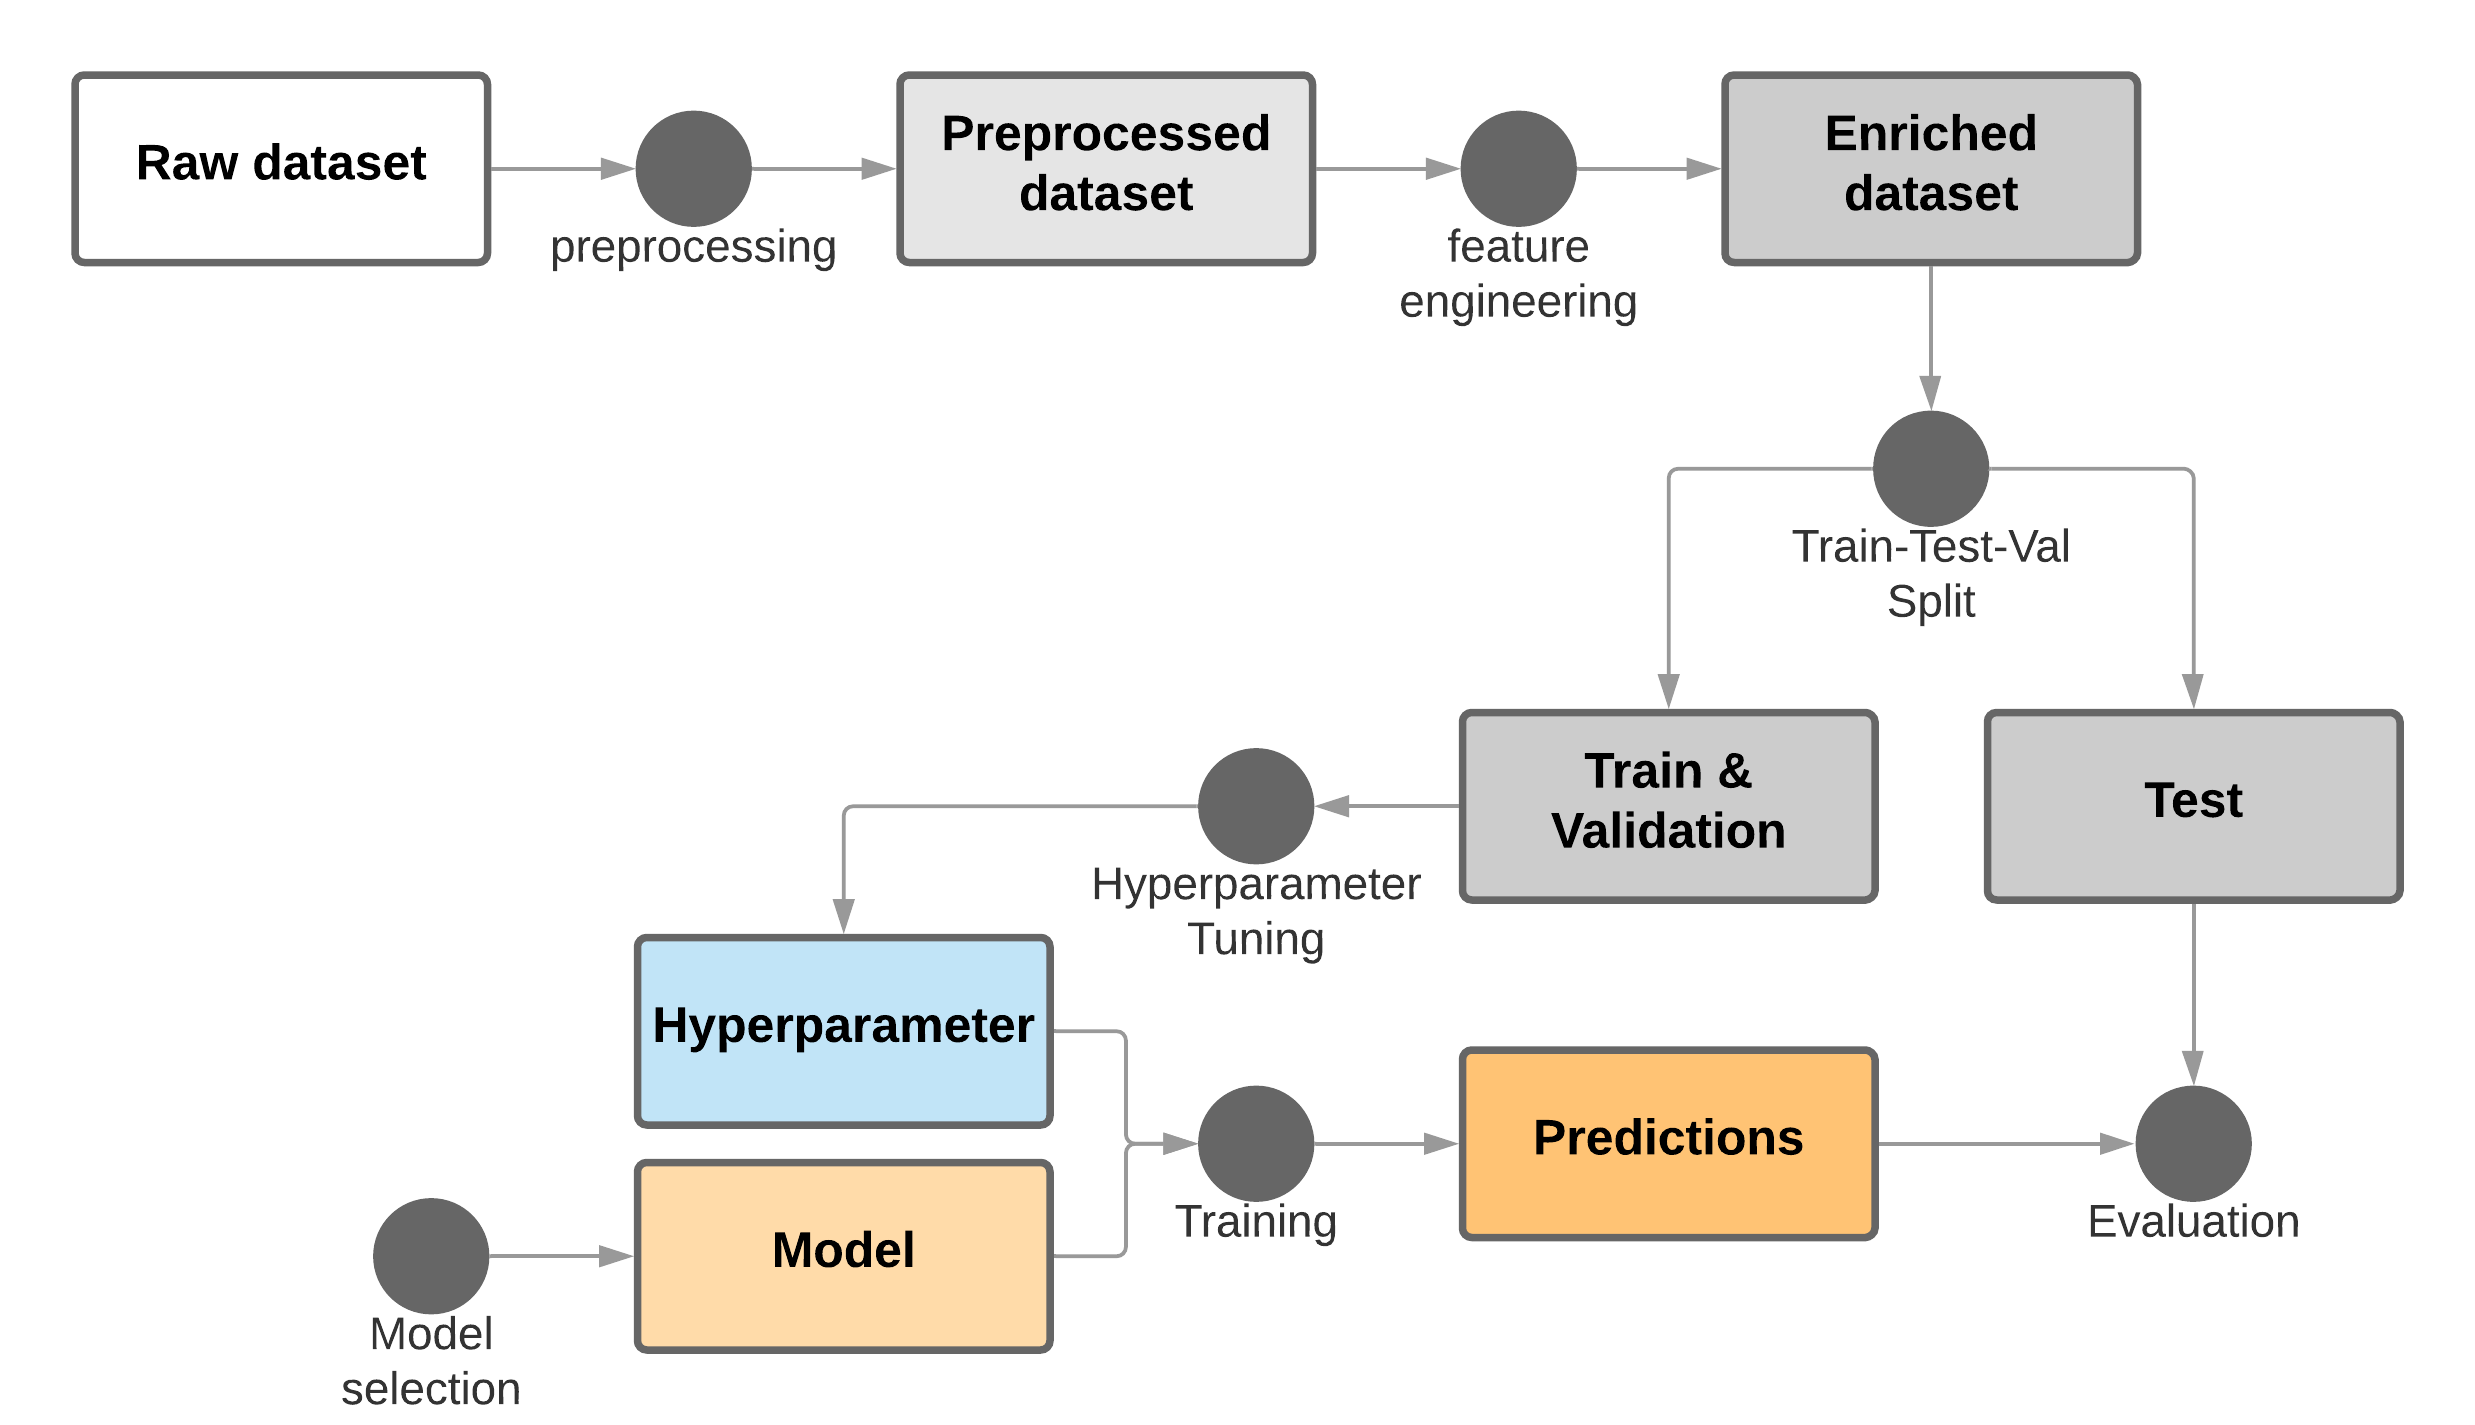
\includegraphics[width=5.20833in,height=\textheight]{images/chapter2/training_cycle.png}
\caption{Iterative Machine Learning lifecycle}\label{fig:ml_cycle}
}
\end{figure}

This process from preparing the data and adjusting the parameters can be
seen in figure \ref{fig:ml_cycle} from a more technical perspective.
First, the developer gets the raw dataset, then he preprocesses this
dataset and applies feature engineering to improve it. After it, the
dataset is split into different sets, and the parameters get tuned. At
the same time, a model is getting selected and trained with the training
set and the given parameters. This step is repeatable until the
developer is satisfied with the created model. In the end, the model's
predictions will be evaluated against the test data.

Last, the model needs to be deployed. For that also, the monitoring and
maintenance of the product need to be clarified. This is how the model
can be applied to its business case. The objective is an easy and stable
way to access the new product. The cycle will then be finalized with a
final report and review of the product as well as the process.
{[}\protect\hyperlink{ref-Wirth2000}{39}{]}

With this standardized process of Artificial Intelligence development,
the basics for applying DevOps to them are already existing. In chapter
\ref{sec:devopsai} will be described how these steps can be automated
while simplifying the work for the developer and increasing the
efficiency at the same time based on the principles and practices of
DevOps described in chapter \ref{sec:devops}.

\hypertarget{sec:devopsai}{%
\section{DevOps for Artificial Intelligence}\label{sec:devopsai}}

The new steps described in chapter \ref{sec:aicycle} forces developers
to change not only their development cycle but also the operation.
Additionally, new architectural models like microservices, cloud
technologies like containerization or Kubernetes as well as \acs{SaaS}
as a new Software model as described in chapter \ref{sec:ms12} opens new
possibilities of a scalable, flexible and reliable deployment of
products. All this changes the way of DevOps for Machine Learning / AI,
and not all of the existing principles and practices are applicable any
more or better approaches are imaginable. Based on the common set of
practices and principles of DevOps described in chapter \ref{sec:devops}
in this chapter these principles will be adopted and extended for
applying it to AI development with the help of the new technologies
presented in chapter \ref{sec:ms12}.

First, DevOps for Machine Learning has to follow the principles named in
chapter \ref{sec:devops}. To repeat, these are the following:

\begin{itemize}
\tightlist
\item
  Develop and test against production-like systems
\item
  Deploy with repeatable processes
\item
  Amplify a feedback loop {[}\protect\hyperlink{ref-Sharma2017}{15}{]}
\end{itemize}

Additionally, the four stages - steer, develop, deploy, and operate -
also apply for Machine Learning. To adopt existing principles, these
stages will be passed through, and necessary adoptions or additions will
be made.

The first set - \textbf{steer} - was about management and planning,
which includes Continuous Business Planning, Continuous Improvement, and
Release Planning. All this includes: Tracking the status and the needs
of a project, monitoring a product and getting feedback from the users
as well as tracking the progress of the project to minimize the risks
and be able to react on trends as quickly as possible.

All this also applies to the development of AI and overlaps with the
CRISP-DM process described in chapter \ref{aicycle}. This process
defines \emph{Business Understanding} as the first stage, in which
business goals and objectives should be defined. During this step, the
same practices and tools can help as in traditional software development
as there is no difference in planning and managing the objectives and
release plan of a Machine Learning or a traditional software project.

The difference in the steer phase is that there is an additional step,
which includes understanding the data. This understanding needs a deeper
insight into the business correlations, necessary information, and
context of the data. So, there are two significant differences -

The first is in the roles of the people who handle these steps. This
profound insight of the business data needs experts on this field
instead of programmers with a lack of understanding all the correlations
and meanings. Instead, usually, data scientists or data analysts are
needed for defining the needed data, evaluating the quality and
detecting problems, so that a clear way to clean and prepare the data
can be determined.ro

A second difference is a need for a tool to visualize these data. For
that, the data scientists or analysts need skills for creating
visualized data as quickly as possible. A widespread tool for this is
\emph{Jupyter Notebooks}, with which an easy preparation and plotting of
the data are possible with the help of Python.

However, most differences are in the \textbf{development and testing}
stage. While in traditional software development this step consists
mainly of coding and testing the single components with unit tests as
well as integration tests, in ML development this stage is split into
two stages - data preparation and the building of the model. Also, the
code is not the only input the developers have to deal with, but there
is data as a second, valuable input.
{[}\protect\hyperlink{ref-Dillon}{9}{]} This leads to several
differences in the practices and tools defined for this stage.

Starting with the \emph{Collaborative development} and \emph{Continuous
integration}, the main point is to integrate and share not only the code
between all participators but also the data. Usual source control
software like git sets limitations to the file size and are not designed
for handling other data than code. This results in need of another tool
to handle big data samples when developing an AI product so that
developers can share and integrate all of their work and not only the
code. This is also necessary to share the results with the client and
keep the product reproducible.

A solution to this problem could be Quilt or Git \acl{LFS} (\acs{LFS}),
which are designed for storing audio samples, graphics, datasets, and
videos.

Another common tool for developing software are IDEs, which are
supporting the developer in coding, collaborating with one's team, and
efficiently integrating the workflow. For Machine Learning, such tools
have to be extended, or new tools need to be created to visualize and
especially prepare data. This includes, for example, possibilities to
label images or videos and preprocess the data. Currently, for this,
different tools have to be used. As long as there is no standardized way
for labeling data, teams should agree on one tool for guaranteeing the
correctness and uniformity.

However, tools for labeling data, managing its quality and collaborating
with a team are emerging. An example is Labelbox, to name just one,
which offers simple data labeling and management, collaboration, and
even some automation features. This labeled and prepared data then needs
to be available from a shared repository, to which the whole team can
contribute to so that they can collaborate.

Another practice in traditional Software development is called
\emph{Continuous testing}. This practice includes automatically build
the software and run unit tests on every single component as well as
automated integration tests of the application as a whole. In AI
development, a completely different form of testing is necessary:

First, a Machine Learning model can only be tested as a whole instead of
its single components. Machine Learning models work more like a black
box because it is difficult to look at how the inner components are
working and evaluate its actions. This means that only an input can be
given and the output can be classified as true or false without a
valuation of the single components.

Additionally, if the output is correct for one input that does not give
any information about another input, because usually, ML models are too
complex to predict its outcome. Both of it leads to another form of
testing.

For this approach, the data needs to be split automatically into a
training and a test set before training the model. After the training
step is done, the test set is used to compare the predicted outcome with
the real value. Applying this approach can give valuable insights into
the model, which can be expressed as different indicators.

The easiest one is the accuracy, which divides the correct classified
results by all tested samples:

\begin{equation}

Accuracy := \frac{\mbox{number of correct predictions}}{\mbox{number of all predictions}}

\end{equation}

Another indicator is a confusion matrix. A confusion matrix shows the
number of \emph{True Positives} and \emph{True Negatives}, which states
correctly predictes positive or negative values, as well as \emph{False
Positives} and \emph{False Negatives}, which states falsely predicted
values. An example can be seen below:

\begin{table}[htb]

\centering

\small

\caption{Example confusion matrix [@aditamishra]}

\begin{tabular}{ c | c | c  }

n=165 &\textbf{Predicted Positive} &\textbf{Predicted Negative} \ \hline

\textbf{Actual Negative} & 50 & 10  \

\textbf{Actual Positive} & 5 & 100 \

\end{tabular}

\end{table}

A third indicator is the F1 score, which first calculates the precision
as well as the recall of a model. Precision is the number of correctly
predicted positive results divided by the number of predicted positive
results. Recall on the other hand is the number of correctly predicted
positive results divided by the number of all samples. The F1 scores
combines those two values to find a balance between them. The greater
the F1 score, the better the performance of the model:

\begin{equation}

\begin{aligned}

Precision &= \frac{\mbox{TruePositives}}{\mbox{TruePositives} + \mbox{FalsePositives}}\

Recall &= \frac{\mbox{TruePositives}}{\mbox{TruePositives} + \mbox{FalseNegatives}}\

F1 &= 2 * \frac{1}{\frac{1}{Precision}+\frac{1}{Recall}}

\end{aligned}

\end{equation}

Last, also the mean squared error can be used as a measure for the
performance of a model. The mean squared error calculates the average of
the differences between the real value and the predicted value:

\begin{equation}

MSE := \frac{1}{N} * \sum*{j=1}^{N}{(y_j - \hat{y}*j)^2}

\end{equation}

However, there are still several other indicators that can be used for
measuring the performance of a model. The developer should decide which
indicators to use, so that they will be seen to evaluate the performance
of a model after the automated tests have been driven.

During the modeling stage, another important difference occurs: The
urgent need for resources, especially of computing units and memory. In
opposite to traditional Software development, this use does not equal
the need for resources while running the application in production, but
it needs far more resources to train the model. Usually, \acs{GPU}s are
used to build models because their design fits the need for model
training better. However, \acs{GPU}s are not very common in traditional
Software development, so teams would have to purchase one just for this
purpose. Additionally, these resources are only needed during the
modeling stage, and the rest of the time, they would be unused, which is
a waste of resources. This is where the advantages of Cloud Computing
can be utilized. With its capability of flexible resource allocation,
the resources can be used more efficiently, and money can be saved
because of the pay-per-use model of Cloud Computing. This approach of
saving cost and resources through training the model within a Cloud can
be called \emph{Dynamical resource demand}.

The next stage is the \textbf{delivery}, in which the practice
\emph{Continuous delivery} applies. This practice deals with the
automation of the deployment of the software to different environments.
This demand also applies to Machine Learning development. Only the
implementation differs slightly. In common Software development, the
trigger for starting the building and deployment process is usually a
newly committed code in the master repository. In Machine Learning, it
could also be necessary or recommended to rebuilt and deploy the model
when new or changed data occurs, which forces a second trigger.
Additionally, the built of the project requires more steps than just
compiling the code like training the model, which takes some time. This
is described in more detail below when it comes to delivery pipelines.

An essential practice during the delivery stage to guarantee the
principle of developing and testing against production-like systems is
to containerize the ML applications and its contents. This guarantees a
consistent environment during all stages, because the containers provide
their environments on their own. The containers can then be deployed in
any system, whether local or Cloud and the results should stay the same.
This is already pretty common for traditional software but is often
avoided with Machine Learning applications because of missing Cloud
computing options. This is why Cloud providers are forced to build Cloud
platforms, that enable the use of \acs{GPU}s on a cluster so that
containerized ML applications can become a reality. This would speed up
the development of ML applications as well as it would increase its
efficiency and reduce costs due to more comfortable ways of building,
testing, and deploying these applications.

Last, there is the \textbf{operation} stage. During this stage, the use
of the application should be monitored, and feedback should be
collected. That information should then be used to improve future
products and support the current version with updates and bugfixes.

For ML applications, this monitoring and feedback get one more,
significant role - through the collection of more data, the model can be
continuously improved through \emph{Refitting of the model}. This is an
exclusive feature for ML applications because, in the opposite of
traditional software, these are adaptive. This demands a clean
collection of the data as well as automated processing of these. Then
this data can be used to retrain the model and redeploy it after
periodically. This offers the users to experience a significant
improvement of the app's performance, and that way increases the User
experience due to better results.

Another critical difference is the roles of developing people. While in
traditional development, the developers are IT specialists, who can
handle the operational cycle as well as the development. In ML
development, usually, Data Scientists take over the main part of the
work as already mentioned above. They got a unique skill set when it
comes to the preparation of data and feature engineering, but sometimes
they lack in experience with operation tools like delivery pipelines.
That is why a more natural way to build and operate a pipeline is
necessary, which can be easily handled and reused so that the process of
development is as easy as possible and the Data Scientist can focus on
his main work with the data.

An essential part of a solution is to provide an easy-to-use delivery
pipeline for the Data Scientists, which combines every step of the
development and automates all the operations as far as possible so that
the Data Scientist can focus on his main work.

An example draft of such a pipeline can be seen in figure
\{fig:devopsaipipeline\}.

\begin{figure}
\hypertarget{fig:devops_architecture}{%
\centering
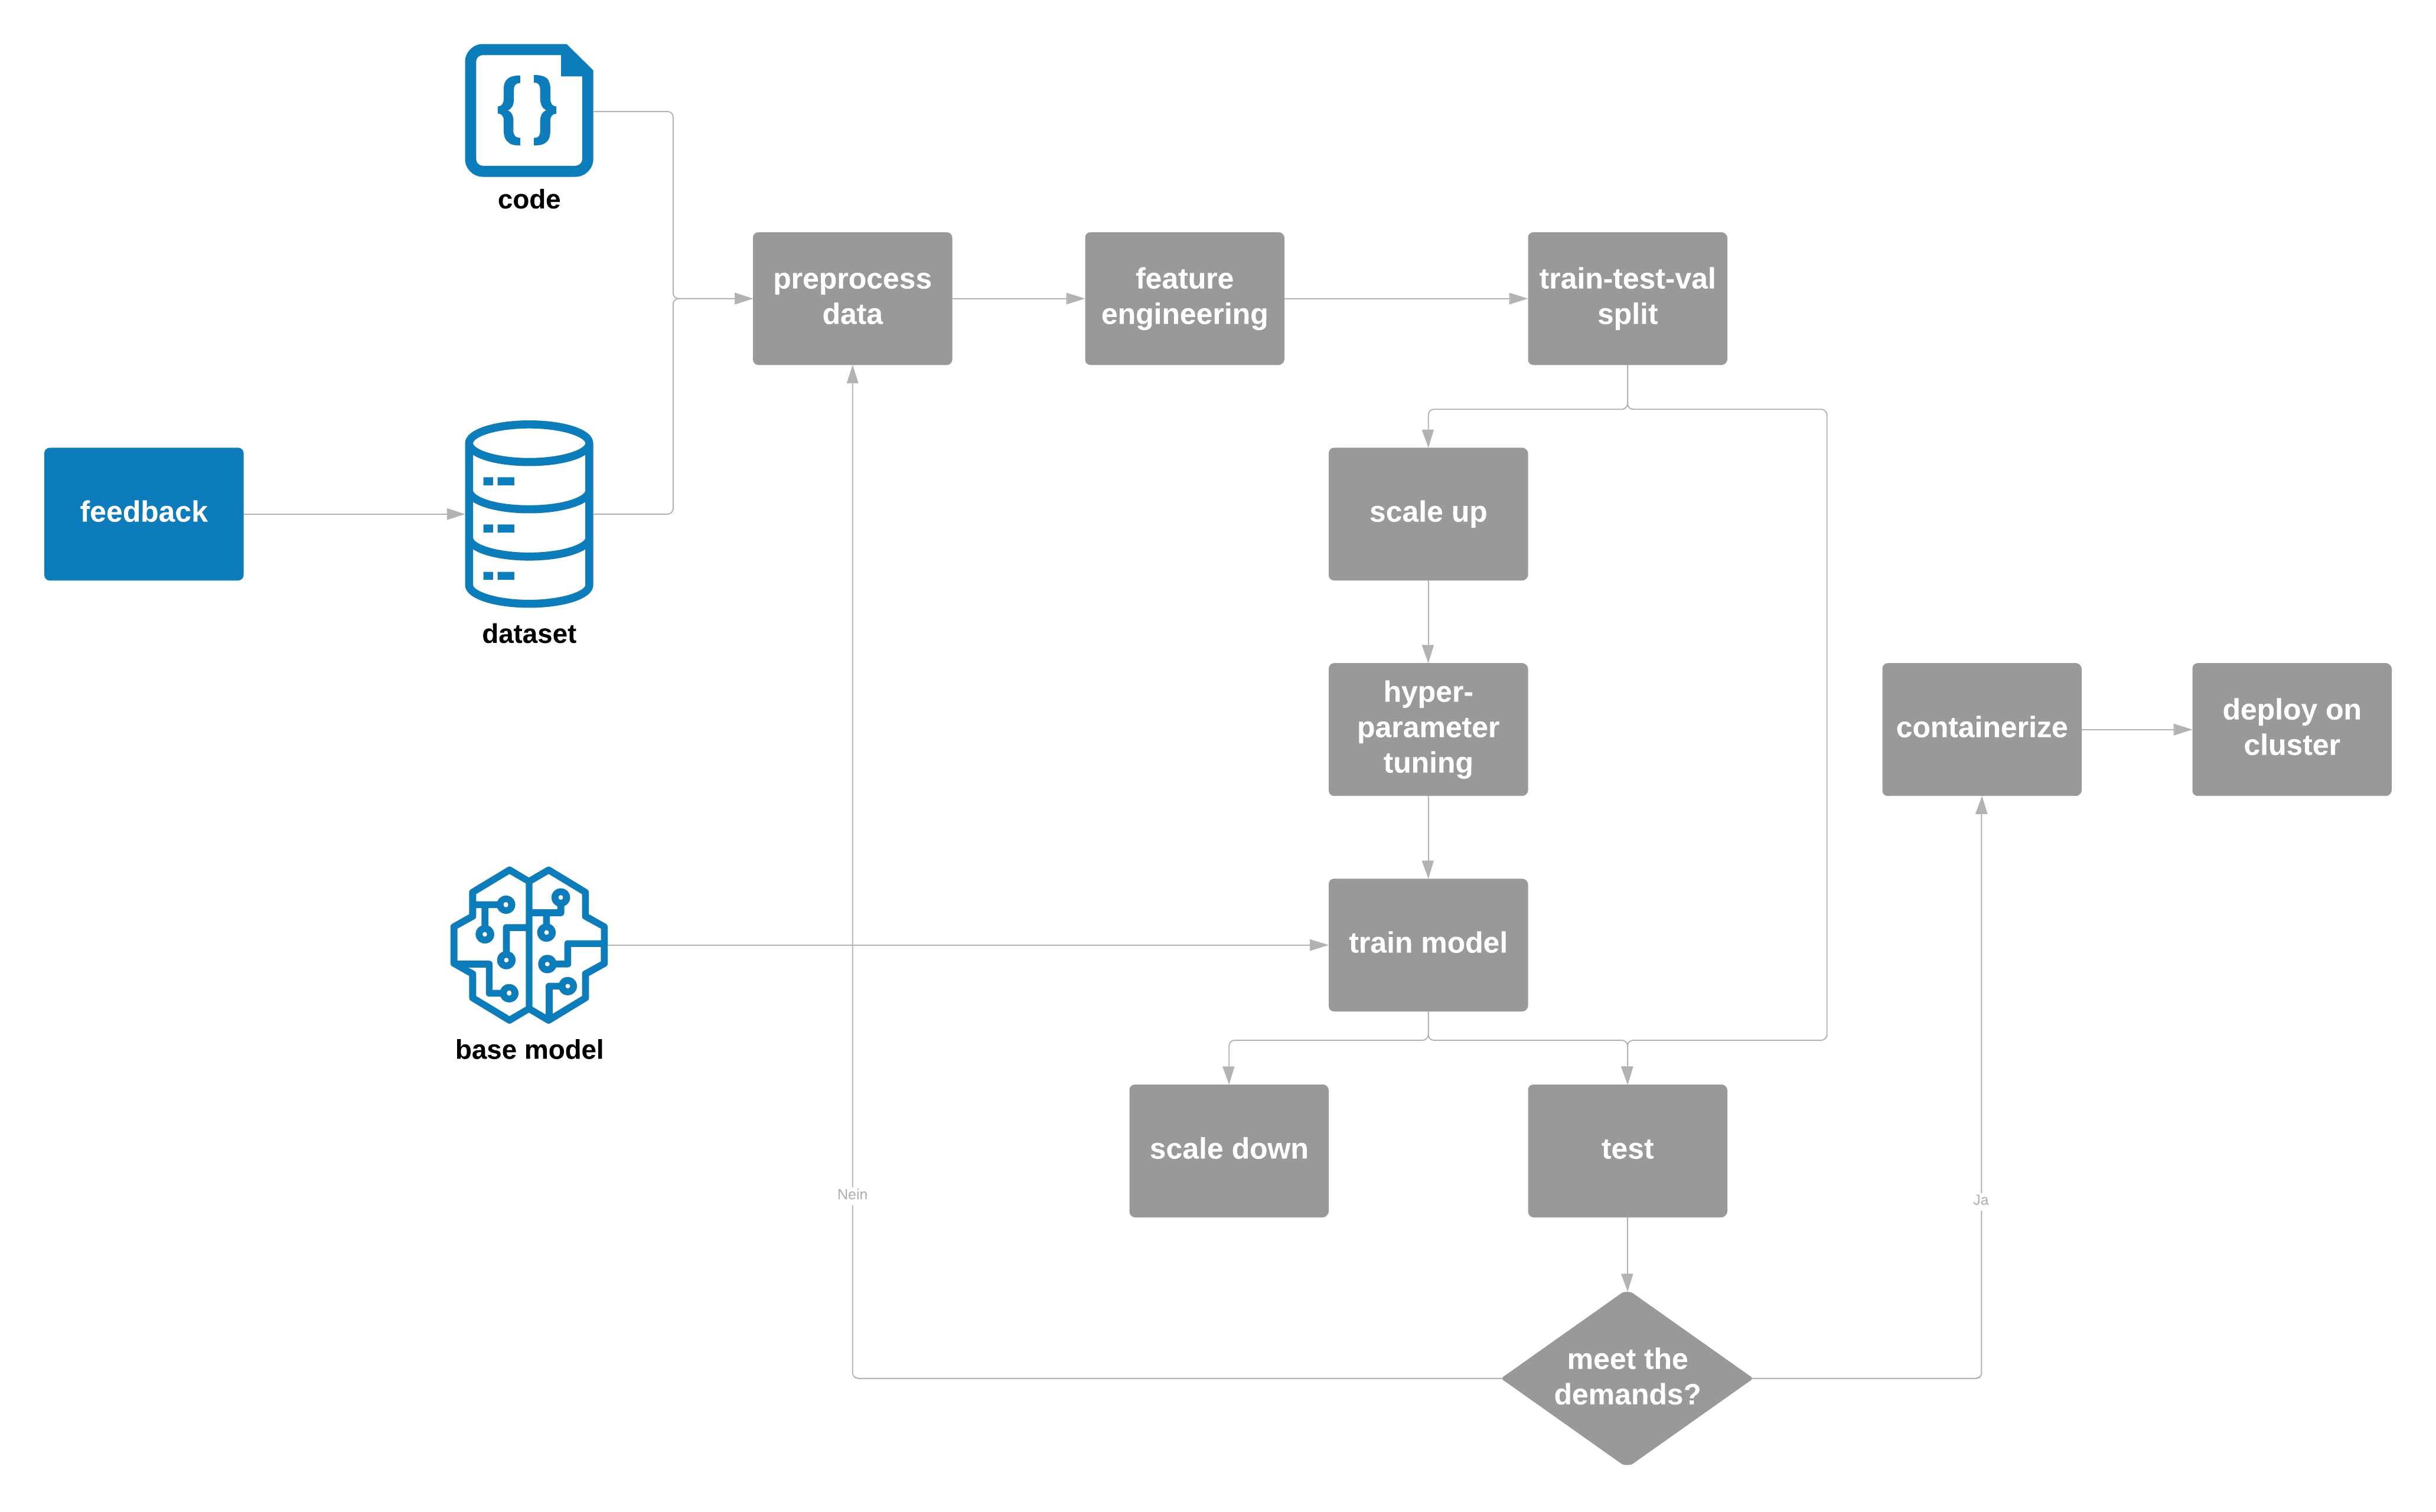
\includegraphics[width=5.20833in,height=\textheight]{images/chapter2/devops_ai_pipeline.png}
\caption{Example devops pipeline}\label{fig:devops_architecture}
}
\end{figure}

There the first difference to traditional DevOps pipelines is, that
there is another input than only the code. This is mainly the data, but
also a base model, on which the model will be trained on. Both of them
can optionally serve as a trigger for starting the delivery process.
Alternatively, the process can be sequentially executed or bumped by the
developers by purpose.

Then there are a preprocessing as well as a feature engineering step.
These two steps are realized by some scripts of the developers, which
take over the preprocessing and feature engineering automatically. The
cleaning and every other necessary step to be made with the data has to
be done manually before pushing the data to its repository.

After this, the dataset is split into three sets - training, validation,
and test. The training and validation sets are then used for the
training of the model, while the test set is only used to test the
finished model at the end.

However, before the training of the model, the pipelines scales up the
cluster, so that enough resources for the training step are available.
Also, the hyperparameter tuning can be done by automated scripts here.
Alternatively, those hyperparameters can be given by input parameters
before the pipeline is executed.

For the training of the model, which takes the main part of the time,
the pipeline usually uses a given basic model, on which the model will
be based on. This is done because building a completely new model from
scratch needs much time and huge amounts of data, which is the reason
why most models are based on some pretrained basic models and only some
are built from scratch.

After this is being done, the cluster can scale down again, and the
model can be tested with the test set. If the results are satisfying,
the model and its application can get containerized automatically and
then deployed on the cluster. The developer can define the way of how
the application should be published and accessible from the cluster for
the end-users. In case the model does not meet the requirements the data
needs or the code needs to be adjusted or cleaned, or different
hyperparameters should be chosen, so that a better model will be built
in the next try.

Last it is to mention, that through feedback given by the users during
the operation stage, the dataset is continuously extended by new data.
This is why the pipeline should repeat the model building sequentially
so that these new data can be used to improve the application
continuously.

With these adjusted and complemented practices above as well as with a
delivery pipeline similar to the described one, the principles of DevOps
can be kept. Through the automated containerization and deployment on a
cluster, every environment can look exactly like the production
environment. If the whole pipeline and application should be tested
first locally before deploying it on a Cloud, it can be tested on a
local Kubernetes cluster like Minikube, which will be described in
chapter \ref{sec:minikube}.

Also, the delivery pipeline guarantees a repeatable and reliable
deployment, in which almost every step can be automated, and the Data
Scientist can focus on his work with the data. The only thing the
developers need to do is providing scripts for an automated
preprocessing and feature engineering if necessary.

The monitor and feedback principle has an even higher importance because
through this, the application can be continuously improved through
feeding the system with the newly gained knowledge.

This is why such a pipeline has significant importance in DevOps for AI.
In the next chapters, two different approaches to building such a
pipeline will be presented and evaluated with previously defined
criteria.

\hypertarget{sec:result}{%
\chapter{Result - Pipeline Creation}\label{sec:result}}

\hypertarget{sec:kubeflowpip}{%
\section{Kubeflow pipeline}\label{sec:kubeflowpip}}

\hypertarget{sec:azurepip}{%
\section{Azure pipeline}\label{sec:azurepip}}

\hypertarget{sec:pip3}{%
\section{Other framework?}\label{sec:pip3}}

\hypertarget{sec:discussion}{%
\chapter{Discussion}\label{sec:discussion}}

\hypertarget{sec:pipelineeval}{%
\section{Pipeline comparison}\label{sec:pipelineeval}}

\hypertarget{sec:outlook}{%
\section{Outlook}\label{sec:outlook}}

\hypertarget{appendix}{%
\chapter{Appendix}\label{appendix}}

placeholder

\hypertarget{bibliography}{%
\chapter*{Literature}\label{bibliography}}
\addcontentsline{toc}{chapter}{Literature}

\hypertarget{refs}{}
\leavevmode\hypertarget{ref-JanakiramMSV}{}%
1. JANAKIRAM MSV. Three Factors That Accelerate The Rise Of Artificial
Intelligence. \emph{2018-05-27} {[}online{]}. Available from:
\url{www.forbes.com/sites/janakirammsv/2018/05/27/here-are-three-factors-that-accelerate-the-rise-of-artificial-intelligence/\%7B/\#\%7D4349a30badd9}

\leavevmode\hypertarget{ref-MichaelShirer}{}%
2. MICHAEL SHIRER and MARIANNE D'AQUILA. Worldwide Spending on
Artificial Intelligence Systems Will Grow to Nearly \$35.8 Billion in
2019. \emph{2019-03-11} {[}online{]}. Available from:
\url{www.idc.com/getdoc.jsp?containerId=prUS44911419}

\leavevmode\hypertarget{ref-MariyaYao}{}%
3. MARIYA YAO. 6 Ways AI Transforms How We Develop Software.
\emph{2018-04-18} {[}online{]}. Available from:
\url{www.forbes.com/sites/mariyayao/2018/04/18/6-ways-ai-transforms-how-we-develop-software/\%7B/\#\%7D1ee109f026cf}

\leavevmode\hypertarget{ref-AndrejKarpathy}{}%
4. ANDREJ KARPATHY. Software 2.0. \emph{2017-11-11} {[}online{]}.
Available from: \url{medium.com/@karpathy/software-2-0-a64152b37c35}

\leavevmode\hypertarget{ref-ArmbrustA.FoxandR.Griffith2009}{}%
5. ARMBRUST, A. FOX, AND R. GRIFFITH, M. Above the clouds: A Berkeley
view of cloud computing. \emph{University of California, Berkeley, Tech.
Rep. UCB} {[}online{]}. 2009.
DOI~\href{https://doi.org/10.1145/1721654.1721672}{10.1145/1721654.1721672}.
Available from: \url{http://arxiv.org/abs/0521865719\%209780521865715}

\leavevmode\hypertarget{ref-Jonas2019}{}%
6. JONAS, Eric, SCHLEIER-SMITH, Johann, SREEKANTI, Vikram, TSAI,
Chia-Che, KHANDELWAL, Anurag, PU, Qifan, SHANKAR, Vaishaal, CARREIRA,
Joao, KRAUTH, Karl, YADWADKAR, Neeraja, GONZALEZ, Joseph, ADA POPA,
Raluca, STOICA, Ion and A. PATTERSON, David. \emph{Cloud Programming
Simplified: A Berkeley View on Serverless Computing}. 2019.

\leavevmode\hypertarget{ref-Amazon}{}%
7. AMAZON DOCUMENTATION. \emph{AWS Lambda -- Serverless Compute - Amazon
Web Services} {[}online{]}. {[}Accessed~25~July~2019{]}. Available from:
\url{aws.amazon.com/lambda/}

\leavevmode\hypertarget{ref-BhagyashreeR}{}%
8. BHAGYASHREE R. How Serverless computing is making AI development
easier. \emph{2018-09-12} {[}online{]}. Available from:
\url{hub.packtpub.com/how-serverless-computing-is-making-ai-development-easier/}

\leavevmode\hypertarget{ref-Dillon}{}%
9. DILLON. CI/CD for Machine Learning \& AI. \emph{2018-10-22}
{[}online{]}. Available from:
\url{blog.paperspace.com/ci-cd-for-machine-learning-ai/}

\leavevmode\hypertarget{ref-DavidLinthicum}{}%
10. DAVID LINTHICUM. DevOps is dictating a new approach to cloud
development. {[}online{]}. Available from:
\url{techbeacon.com/app-dev-testing/devops-dictates-new-approach-cloud-development}

\leavevmode\hypertarget{ref-SusanMoore2019}{}%
11. SUSAN MOORE. \emph{How to Get Started With AIOps} {[}online{]}.
Gartner, 2019. Available from:
\url{www.gartner.com/smarterwithgartner/how-to-get-started-with-aiops/}

\leavevmode\hypertarget{ref-Pugh:2002:OSB:513126.513131}{}%
12. PUGH, Emerson W. Origins of Software Bundling. \emph{IEEE Ann. Hist.
Comput.} {[}online{]}. 2002. Vol.~24, no.~1, p.~57--58.
DOI~\href{https://doi.org/10.1109/85.988580}{10.1109/85.988580}.
Available from: \url{http://dx.doi.org/10.1109/85.988580}

\leavevmode\hypertarget{ref-SteveMezak}{}%
13. STEVE MEZAK. The Origins of DevOps: What's in a Name?
\emph{2018-01-25} {[}online{]}. Available from:
\url{https://devops.com/the-origins-of-devops-whats-in-a-name/}

\leavevmode\hypertarget{ref-SauceLabs}{}%
14. SAUCE LABS. \emph{Extent of DevOps adoption by software developers
in 2017 and 2018} {[}online{]}. Available from:
\url{www.statista.com/statistics/673505/worldwide-software-development-survey-devops-adoption/}

\leavevmode\hypertarget{ref-Sharma2017}{}%
15. SHARMA, Sanjeev and COYNE, Bernie. \emph{DevOps for Dummies}. 3rd
IBM Li. John Wiley \& Sons, 2017.
ISBN~\href{https://worldcat.org/isbn/978-1-119-41589-3}{978-1-119-41589-3}.

\leavevmode\hypertarget{ref-IBM2013}{}%
16. IBM. Continuous Business Planning - Connecting the dots between
strategy and execution. In~: \emph{Innovate2013}. 2013.

\leavevmode\hypertarget{ref-AmazonDocumentation}{}%
17. AMAZON DOCUMENTATION. \emph{What is Continuous Integration? --
Amazon Web Services} {[}online{]}. Available from:
\url{https://aws.amazon.com/devops/continuous-integration/}

\leavevmode\hypertarget{ref-TaliSoroker}{}%
18. TALI SOROKER. \emph{3 Reasons Why Version Control is a Must for
Every DevOps Team} {[}online{]}. Available from:
\url{https://blog.overops.com/3-reasons-why-version-control-is-a-must-for-every-devops-team/}

\leavevmode\hypertarget{ref-MileciaMcG}{}%
19. MILECIA MCG. Difference Between Development, Stage, And Production.
\emph{2019-04-30} {[}online{]}. Available from:
\url{https://dev.to/flippedcoding/difference-between-development-stage-and-production-d0p}

\leavevmode\hypertarget{ref-Debbie}{}%
20. DEBBIE. The staging environment vs test environment: What's the
difference? \emph{2018-08-01} {[}online{]}. Available from:
\url{https://www.plesk.com/blog/product-technology/staging-environment-vs-test-environment/}

\leavevmode\hypertarget{ref-Kumar2014}{}%
21. KUMAR, K. V. K Mahesh. SOFTWARE AS A SERVICE FOR EFFICIENT CLOUD
COMPUTING. \emph{International Journal of Research in Engineering and
Technology} {[}online{]}. 2014. Available from:
\url{https://pdfs.semanticscholar.org/4160/859c66dc8809a1829d2d83d69b079c545300.pdf}

\leavevmode\hypertarget{ref-MartinFowler}{}%
22. MARTIN FOWLER and JAMES LEWIS. Microservices - a definition of this
new architectural term. \emph{2014-03-25} {[}online{]}. Available from:
\url{https://martinfowler.com/articles/microservices.html}

\leavevmode\hypertarget{ref-Wiggins}{}%
23. WIGGINS, Adam. \emph{The Twelve-Factor App} {[}online{]}.
{[}Accessed~22~August~2019{]}. Available from:
\url{https://12factor.net/}

\leavevmode\hypertarget{ref-Jerry2015}{}%
24. JERRY, Preissler and TIGGES, Oliver. Docker - perfekte Verpackung
von Microservices. \emph{OBJEKTspektrum} {[}online{]}. 2015. Available
from:
\url{https://www.sigs-datacom.de/uploads/tx\%7B/_\%7Ddmjournals/preissler\%7B/_\%7Dtigges\%7B/_\%7DOTS\%7B/_\%7DArchitekturen\%7B/_\%7D15.pdf}

\leavevmode\hypertarget{ref-Mikesir87}{}%
25. MIKESIR87. Docker is NOT a Hypervisor. \emph{2017-05-08}
{[}online{]}. Available from:
\url{https://blog.mikesir87.io/2017/05/docker-is-not-a-hypervisor/}

\leavevmode\hypertarget{ref-DockerDocumentation}{}%
26. DOCKER DOCUMENTATION. \emph{Docker security} {[}online{]}.
{[}Accessed~22~August~2019{]}. Available from:
\url{https://docs.docker.com/engine/security/security/}

\leavevmode\hypertarget{ref-Lipke2017}{}%
27. LIPKE, Simon. \emph{Building a Secure Software Supply Chainusing
Docker} {[}online{]}. PhD thesis. 2017. Available from:
\url{https://hdms.bsz-bw.de/frontdoor/deliver/index/docId/6321/file/20170830\%7B/_\%7Dthesis\%7B/_\%7Dfinal.pdf}

\leavevmode\hypertarget{ref-NoahZoschke}{}%
28. NOAH ZOSCHKE. Modern Twelve-Factor Apps With Docker.
\emph{2015-05-18} {[}online{]}. Available from:
\url{https://medium.com/@nzoschke/modern-twelve-factor-apps-with-docker-55dd92c832b3}

\leavevmode\hypertarget{ref-Fricke}{}%
29. FRICKE, Thomas. Kubernetes: Architektur und Einsatz -- Einführung
mit Beispielen \textbar{} Informatik Aktuell. \emph{2018-01-16}
{[}online{]}. Available from:
\url{https://www.informatik-aktuell.de/entwicklung/methoden/kubernetes-architektur-und-einsatz-einfuehrung-mit-beispielen.html}

\leavevmode\hypertarget{ref-CoreOS}{}%
30. COREOS. \emph{Overview of Pods} {[}online{]}.
{[}Accessed~22~August~2019{]}. Available from:
\url{http://coreos.com/kubernetes/docs/latest/pods.html}

\leavevmode\hypertarget{ref-JorgeAcetozi}{}%
31. JORGE ACETOZI. Kubernetes Master Components: Etcd, API Server,
Controller Manager, and Scheduler. \emph{2017-12-11} {[}online{]}.
Available from:
\url{https://medium.com/jorgeacetozi/kubernetes-master-components-etcd-api-server-controller-manager-and-scheduler-3a0179fc8186}

\leavevmode\hypertarget{ref-MichaelD.Elder}{}%
32. MICHAEL D. ELDER. Kubernetes \& 12-factor apps. \emph{2019-05-03}
{[}online{]}. Available from:
\url{https://medium.com/ibm-cloud/kubernetes-12-factor-apps-555a9a308caf}

\leavevmode\hypertarget{ref-Mitchell:1997:ML:541177}{}%
33. MITCHELL, Thomas M. \emph{Machine Learning}. 1. New York, NY, USA~:
McGraw-Hill, Inc., 1997.
ISBN~\href{https://worldcat.org/isbn/0070428077,\%209780070428072}{0070428077, 9780070428072}.

\leavevmode\hypertarget{ref-Goodfellow-et-al-2016}{}%
34. GOODFELLOW, Ian, BENGIO, Yoshua and COURVILLE, Aaron. \emph{Deep
Learning}. MIT Press, 2016.

\leavevmode\hypertarget{ref-AmnahKhatun}{}%
35. AMNAH KHATUN. Let's know Supervised and Unsupervised in an easy way.
\emph{2018-07-10} {[}online{]}. Available from:
\url{https://chatbotsmagazine.com/lets-know-supervised-and-unsupervised-in-an-easy-way-9168363e06ab}

\leavevmode\hypertarget{ref-Stroetmann2018}{}%
36. STROETMANN, Karl. \emph{An Introduction to Artificial Intelligence}
{[}online{]}. 2018. Available from:
\url{https://github.com/karlstroetmann/Artificial-Intelligence/blob/master/\%7B/\%\%7D0ALecture-Notes/artificial-intelligence.pdf}

\leavevmode\hypertarget{ref-VictorZhou}{}%
37. VICTOR ZHOU. Machine Learning for Beginners: An Introduction to
Neural Networks. \emph{2019-03-05} {[}online{]}. Available from:
\url{https://towardsdatascience.com/machine-learning-for-beginners-an-introduction-to-neural-networks-d49f22d238f9}

\leavevmode\hypertarget{ref-WolfRiepl}{}%
38. WOLF RIEPL. CRISP-DM: Ein Standard-Prozess-Modell für Data Mining.
\emph{2012-04-09} {[}online{]}. Available from:
\url{https://statistik-dresden.de/archives/1128}

\leavevmode\hypertarget{ref-Wirth2000}{}%
39. WIRTH, Rüdiger. CRISP-DM : Towards a Standard Process Model for Data
Mining. \emph{Proceedings of the Fourth International Conference on the
Practical Application of Knowledge Discovery and Data Mining}. 2000.
DOI~\href{https://doi.org/10.1.1.198.5133}{10.1.1.198.5133}.

\leavevmode\hypertarget{ref-article}{}%
40. KOTSIANTIS, Sotiris, KANELLOPOULOS, Dimitris and PINTELAS, P. Data
Preprocessing for Supervised Learning. \emph{International Journal of
Computer Science}. 2006. Vol.~1, p.~111--117.

\leavevmode\hypertarget{ref-SunnySrinidhi}{}%
41. SUNNY SRINIDHI. Label Encoder vs. One Hot Encoder in Machine
Learning. \emph{2019-07-30} {[}online{]}. Available from:
\url{https://medium.com/@contactsunny/label-encoder-vs-one-hot-encoder-in-machine-learning-3fc273365621}


\end{document}
